\documentclass[titlepage]{article}

%\usepackage{tabto}
\usepackage{tabularx}
\usepackage{graphicx}
\usepackage{longtable}
\usepackage{float}
\usepackage{subfig}
\graphicspath{ {./images/} }


\title{{\Huge {\it Data4Help}}}
\author{Lorenzo, Molteni, Negri}
\date{December 10, 2018}

\begin{document}

\makeatletter
    \begin{titlepage}
        \begin{center}
            
\includegraphics[width=\linewidth]{logo.png}\\[20ex]
            {\huge  \@title }\\[2ex] 
            {\LARGE  \@author}\\[3ex] 
            {\LARGE {\it DD} - Design Document}\\[3ex]
            {\large \@date}\\[5ex]
        \end{center}
    \end{titlepage}
\makeatother
\thispagestyle{empty}
\newpage

%Add content for page two here (useful for two-sided printing)
\thispagestyle{empty}
\newpage


	
%Index	
\pagebreak
\tableofcontents{}
\pagebreak

%%%%%%%%%%%%%%%%%%%%%%%%%%%%%%%%%%%%%%%%%%%%%%%%%
%%%%%%%%%%%%%%%%%%%%SECTION 1%%%%%%%%%%%%%%%%%%%%
%%%%%%%%%%%%%%%%%%%%%%%%%%%%%%%%%%%%%%%%%%%%%%%%%
\section{Introduction}
\subsection{Purpose}
This document deals with the architectural description of Data4Help and its services and is the result of successive refinements made together with Stakeholders to satisfy their needs. 
On one hand, developers will find an in-depth description of the components of the System, the interactions between them, their deployment and how they will be implemented.
On the other hand, the QA team will find plans for both unit testing and integration testing.
Finally, requirements expressed in the RASD document will be dealt with here, describing how the components presented can satisfy them.

\subsection{Scope}
As explained in the RASD document, Data4Help is a service whose main purpose is to allow users to keep track of their health status, both on their own and by allowing experts to access their data. It will be available as a mobile application in the italian app stores only. 
Private users can import data from their tracking devices and access it whenever they need, making it possible to analyze the evolution of specific health parameters in time.
Companies can access data of private users by sending them requests or retrieve anonymized data from groups of users who meet certain conditions. All data requested by these Third Parties will be used only for medical purposes.
\newline
\textit{AutomatedSOS} is the first service offered on top of Data4Help, and ensures that an ambulance is called whenever the health parameters of a user fall below a critical threshold, based on his age. The ambulance is provided with the last known position of the user.

\textit{Track4Run} is the second service that uses Data4Help to allow users to create runs, take part in them and spectate their participants. 

\subsection{Definitions, Acronyms, Abbreviations}


	\subsubsection{Definitions}
	
	\begin{itemize}
				\item {\bf Client: }Software system on the user’s device that requests services to the Server.
				\item {\bf Server: }Software system that handles requests from different clients.
				\item {\bf n-tier: }Distributed architecture composed of n hardware components, each containing one or many layers.
				\item {\bf n-layer: }Distributed architecture composed of n software levels, each distributed on one or many tiers.
				\item {\bf Design Pattern: }Reusable software solution to a commonly occurring problem within a given context of software design.
				\item {\bf Driver: }a piece of software that simulates a component that depends on the module undergoing testing.
				\item {\bf Stub: }a piece of software that simulates a components on which the module undergoing testing depends.
	\end{itemize}
	
	
	\subsubsection{Acronyms}
	
	\begin{longtable}{| p{2 cm} | p{7 cm} |} \\ \hline
		{\bf MVCS} & Model-View-Controller-Store \\ \hline
		{\bf DBMS} & Data Base Management System \\ \hline
		{\bf REST} & REpresentational State Transfer \\ \hline
		{\bf API} & Application Programming Interface \\ \hline
		{\bf OS} & Operating System\\ \hline
		{\bf UI} & User Interface \\ \hline
		{\bf QA} & Quality Assurance \\ \hline		
		{\bf HTTP} & HyperText Transfer Protocol \\ \hline	
		{\bf TTS} & Text-to-Speech \\ \hline
		\caption{Acronyms}							
	\end{longtable}

	\subsubsection{Abbreviations}
	
	\begin{itemize}
		\item {\bf (Rn):} n-th Requirement
	\end{itemize}
			
			
\subsection{Revision history}

\begin{table}[ht]
	\centering
	\begin{tabular}{ccc} 
		Version & Date & Changes  \\ 
		\hline
		1.1 & 12/11/2018 & Initial draft \\
		1.2 & 10/12/2018 & First deadline draft \\
	\end{tabular}
	\caption{Revision History}
	\label{default}
\end{table}
	
	
\subsection{Reference Documents}

\begin{itemize}
   	\item ISO/IEC/IEEE 29148: https://www.iso.org/standard/45171.html 
	\item Alloy Official Documentation: \\
	http://alloy.lcs.mit.edu/alloy/documentation.html 
   	\item Four Dark Corners of Requirements Engineering – Jackson, Zave 
	\item Project Assignment 
\end{itemize}


\subsection{Document Structure}
The remaining sections of the DD are organized as follow:
    \begin{itemize}
        \item {\bf Architectural Design: }details the system’s architecture by defining the main components and the relationships between them as well as specifying the hardware needed for the system deployment. The last part of this section will also focus on design choices and architectural styles, patterns and paradigms.
		\item {\bf User Interface Design:  }following what has already been included in the RASD this section defines the UX by means of view flow modelling.
		\item {\bf Requirements Traceability: }shows the relations between the requirements from the RASD and the design choices of the DD and how they are satisfied by the latter.
		\item {\bf Implementation, Integration and Test Plan: }provides a roadmapping of the implementation and integration process of all components and explains how the integration will be tested.
		\item {\bf Effort spent: }describes how the work has been split between all members of the team and how long did the DD take to be completed.
    \end{itemize}
\pagebreak


%%%%%%%%%%%%%%%%%%%%%%%%%%%%%%%%%%%%%%%%%%%%%%%%%
%%%%%%%%%%%%%%%%%%%%SECTION 2%%%%%%%%%%%%%%%%%%%%
%%%%%%%%%%%%%%%%%%%%%%%%%%%%%%%%%%%%%%%%%%%%%%%%%

\section{Architectural Design}
\subsection{Overview}

\begin{figure}[H]
	\center
  	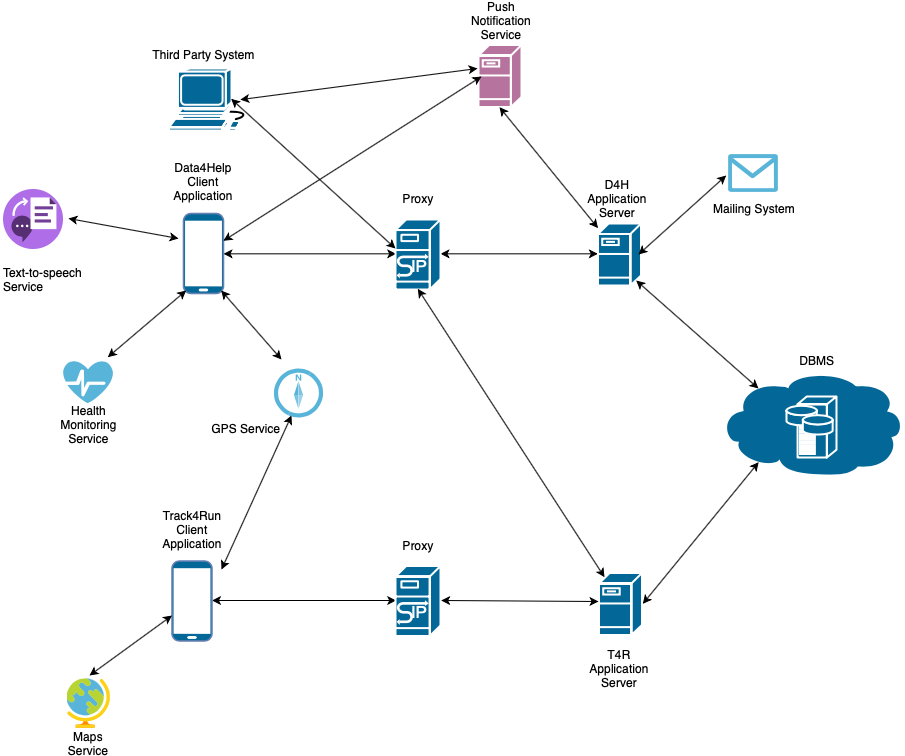
\includegraphics[width=10cm]{Overview.png}
  	\caption{Overview of the System}
 	\label{fig:OVERVIEW}
\end{figure}

The above image provides a general overview of the System’s architecture. We can immediately identify two horizontal layers and four vertical ones.
The horizontal layers correspond to Data4Help and Track4Run’s architectures that while having their own Client Applications, Proxies and Application Servers, they also communicate internally to the System’s server network. 
Precisely, Track4Run accesses Data4Help’s functionalities and integrates them in its services by performing requests to its proxy.
The vertical layers separate the Client side, including Client Applications and Third Party Systems accessing the applications’ APIs, from the Server side, including the Application Servers, the Proxies and from the shared external Database, accessed through its cloud interface.
Finally also all external services are included in the diagram, both those accessed by the Clients, such as Maps, GPS and Health Monitoring services, and those accessed by the Servers, such as a Mailing System and a Push Notification service.
\pagebreak

\subsection{Component view}

\begin{figure}[H]
	\center
  	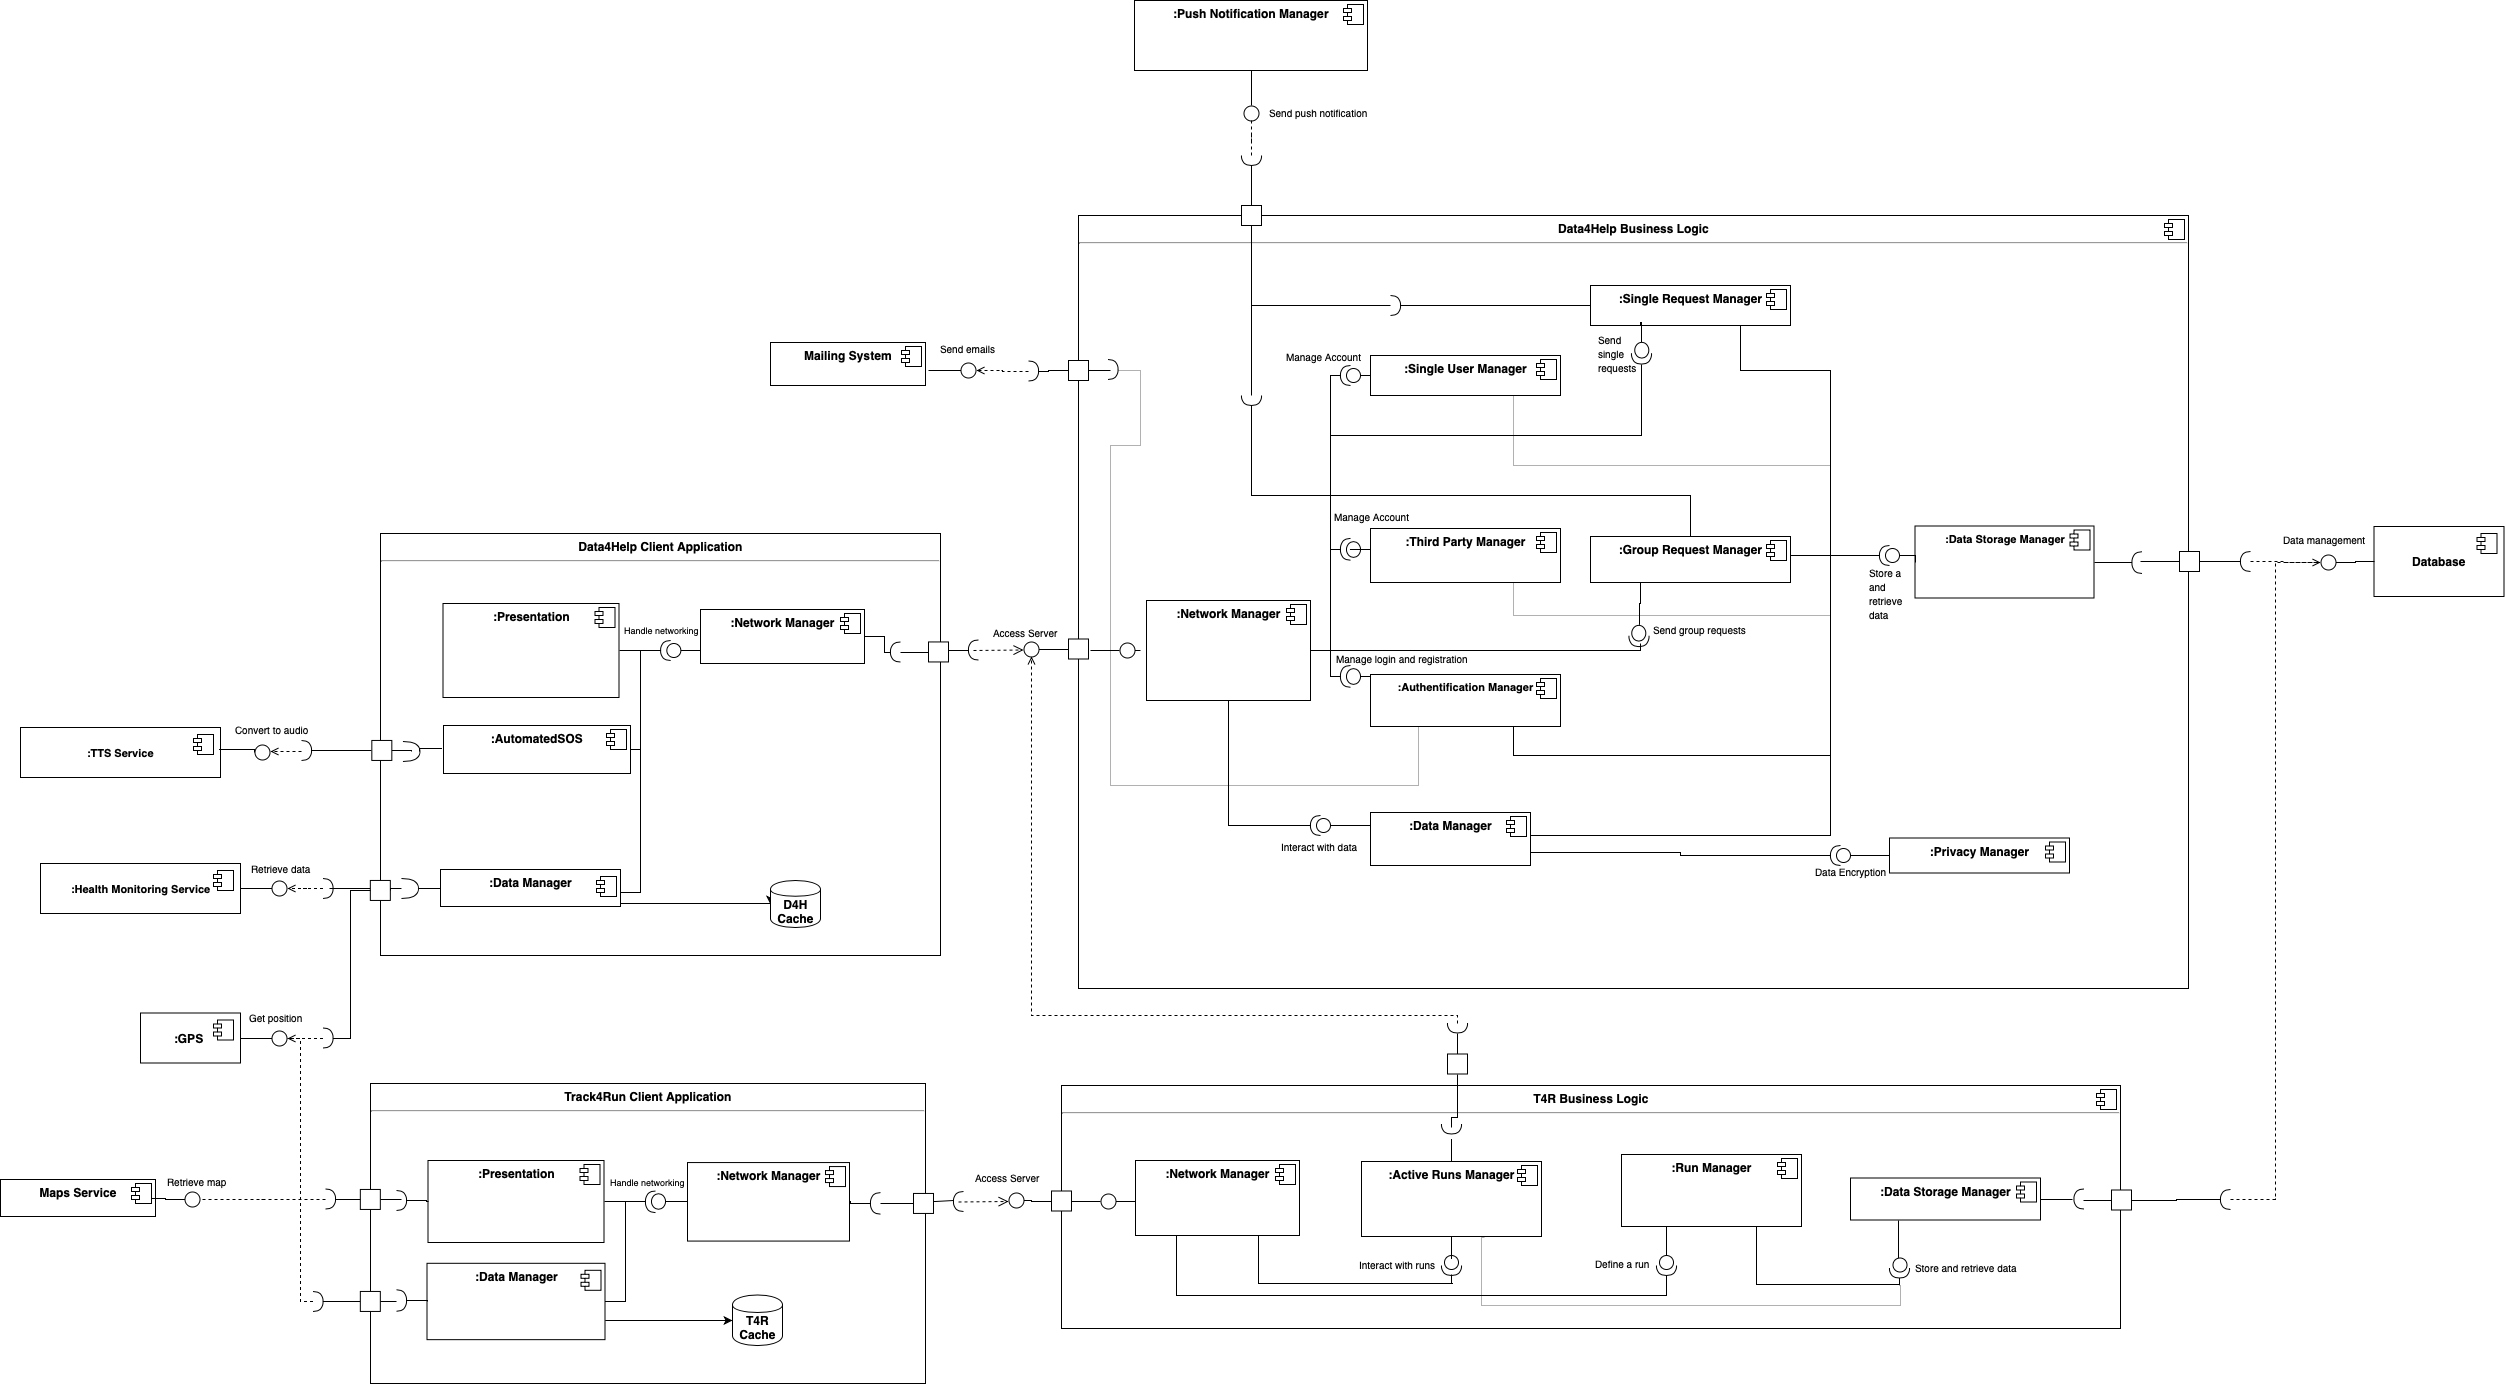
\includegraphics[width=10cm]{ComponentDiagram.png}
  	\caption{Component diagram}
 	\label{fig:COMPDIA}
\end{figure}

The purpose of this UML diagram is to show the internal architecture of the system’s software. It is globally divided into five components: the Data4Help and Track4Run Client Applications, their Business Logic components and the shared external Database. Both business logic components communicate directly with a unique database. However Track4Run’s business layer also accesses Data4Help’s services through its APIs. These main layers are internally organized in modular components, each providing specific services. 
Components communicate with one another other by providing interfaces where they produce information that is used by the required interface of other components. In our diagram, this is represented internally to a component by assembly connectors ball-and-socket and externally by delegation connectors, required interfaces and provided interfaces.
We will now focus on one component at a time and describe its functionalities and relationships with others. 

{\bf Data4Help Client Application }\\ 
This component is located on the user’s device. Its modules are the Network Manager, the Presentation Component, the Data Manager and AutomatedSOS. 
The first component is committed to dispatching all incoming and outgoing communications with the application server. Whenever it receives a request to show to the user, before forwarding it to its handler, the Network Manager sends a push notification.
The Presentation Component corresponds to the “View” in the MVCS Pattern. It requires data provided by the business logic component to project it on the User Interface and does not add further functionalities. 
The Data Manager is the module that calls Heath Monitoring Services APIs to import the user’s health data. It gathers data of the required type and forwards it to the requesting application server.
Finally, the last component contains the only portion of logic on the Client Application. It functions in background only if enabled by the user, otherwise remains inactive. Each time the client application imports new health data from the user’s device, before forwarding it to the business component, AutomatedSOS performs a set of controls in order to decide whether an ambulance must be called. 

{\bf Data4Help Business Logic }\\ 
This component is devoted to the implementation of Data4Help’s core logic. It is a stateless module that lies between the Client application and the central Database. It gathers all components that interact with each other to provide the system’s functionalities. We will now detail how each component is structure and what is its purpose.
\begin{itemize}
        \item {\bf Nework Manager }\\
        This component handles all incoming and outgoing messages exchanged between Clients and Server. With respect to incoming the incoming flow, It dispatches all messages received from client applications to the specific handler components in the Business Logic. On the other hand, it gathers all outgoing messages and sends them to the correct Client Application through the unique port.
		\item {\bf Authentication Manager }\\
		The Authentication Manager exposes all methods related to the access to the platform. Specifically, it deals with user registration and login and to do so it continuously interacts with the database through the Data Storage Interface. It handles credentials verification and constraints and guarantees the creation of consistent accounts. Furthermore, in order to confirm to users they have successfully registered, the Authentication Manager sends them an email by accessing the Mailing System’s Interface.
		\item {\bf Single User Manager }\\
		The Single User manager handles all functionalities related to a Single User Account. Its services are directly called from users and performs them by interacting continuously with the Database through the Data Storage Interface. The provided services include settings update, change of password, change of imported data types and retrieval of single users’ Third Party followers.
		\item {\bf Third Party Manager }\\
		The Third Party Manager deals with all services that concern Third Party Accounts. Specifically it exposes methods to update the user’s settings, change its password and retrieve the history of all requests to Single Users. In order to provide these functionalities, this component continuously with the Database through the Data Storage Interface.
		\item {\bf Data Manager }\\
		This component is the main gateway between the Client Applications and the central Database. It handles the import of new data associated to a user’s account and its retrieval, as well as organizing it and evaluating statistics before passing it back to the client who requested it.
		\item {\bf Single Request Manager }\\
		The Single Request Manager handles the creation and management of single requests performed by Third Parties and directed to Single Users. It provides both services to Third Parties, such as the creation of a new request and the retrieval of its response, and to Single Users, such as the possibility to accept or decline a request or to end its subscription.
		\item {\bf Group Request Manager }\\
		This component is devoted to the management of group requests, created by Third Party users and addressed to the system. It offers services such as the creation of group requests and the enabling of subscriptions. Retrieving the result is possible by querying the central Database through the Data Storage Interface.
		\item {\bf Privacy Manager }\\
		The Privacy Manager exposes methods to encrypt sensitive data. This operation is needed in order to store information about users in a secure way in order to reduce the effects of data leaks and to prevent Third Parties from accessing sensitive data with group requests. 
		\item {\bf Data Storage Manager }\\
		The Data Storage Manager provides all methods to interact with the central Database such as data retrieval, storage and update.
    \end{itemize} 
    
{\bf Track4Run Client Application }\\ 
This component consists of the client side of Track4Run’s application. Its architecture is that of a thin client as it doesn’t contain any logic of the system. It is composed of three modules: the Network Manager, that dispatches all incoming and outgoing messages, the Presentation component and the Data Manager, committed to import GPS data required to access the application’s functionalities. 

{\bf Track4Run Business Logic }\\ 
This component is devoted to the implementation of Track4Run’s core logic. While relying on Data4Helps main services such as authentication and account management and its request protocol, Track4Run adds further functionalities to its users thanks to the interaction of Run Manager and Active Runs Manager. 
Interaction with Client Applications and the central Database are handled respectively by the Network Manager and the Data Storage Manager.
We will now detail each component’s inner implementation:
\begin{itemize}
        \item {\bf Nework Manager }\\
        This component is devoted to handling all messages exchanged between business logic and client applications. Messages are received through a unique port and handled by the different business components.
		\item {\bf Run Manager }\\
		Run Manager exposes methods to Third Parties  to create and manage new runs. Runs must be defined by adding an associated path, a duration and brief description. This component interacts with the central database as it needs to store all newly created runs.
		\item {\bf Active Runs Manager }\\
		This component grants access to users to all active runs and enables interaction with them such as the possibility to spectate or join them. Active Runs Manager is also linked to the central database in order to retrieve information about all active runs.
		\item {\bf Data Storage Manager }\\
		This component is the unique point of access to the Database in this tier. It handles all data management operations such as data storage, retrieval and update.
    \end{itemize}

{\bf External Interfaces }\\ 
Some of the described components in our System are also dedicated to communicating with external services through specific interfaces. These communications are bilateral and essential to guarantee the application’s functionalities. These components are both on the Client side and on the server side. We will now describe how each external service used by the system is accessed:
\begin{itemize}
        \item {\bf Database }\\
        The component devoted to interacting with the central database on cloud is the Data Storage Manager. It is interposed between all other business logic modules and the external database. This component is shared by both Track4Run and Data4Help.
		\item {\bf GPS }\\
		On the Client side of the application, both Data4Help and Track4Run access data from the user’s device’s GPS through the Data Managers’ interface. GPS information is essential for both health analysis and data requests in the first application and geolocalization while running in the second.
		\item {\bf Health Monitoring System }\\
		The Data Manager module is also responsible for the retrieval of health data from the user’s device through its interface. This service too is essential for the core functioning of the applications.
		\item {\bf Mailing System }\\
		In order to inform users of having successfully created an account on Data4Help, the Authentication Manager requires access to the Mailing System to send a confirmation email.
		\item {\bf Maps Service }\\
		Access to a mapping service is essential for Track4Run to provide its core functionalities. Access is performed by the Client Application to enable the definition of a path for a run.
		\item {\bf TTS Service }\\
		This service is used when the AutomatedSOS component spots a critical situation for a Private User, and has to call an ambulance. The component prepares a text message containing the coordinates of the user and a brief help statement, and then passes this message to the TTS service to get the audio version, usable in the ambulance call.
    \end{itemize} 

\pagebreak



\subsection{Deployment view}

\begin{figure}[H]
	\center
  	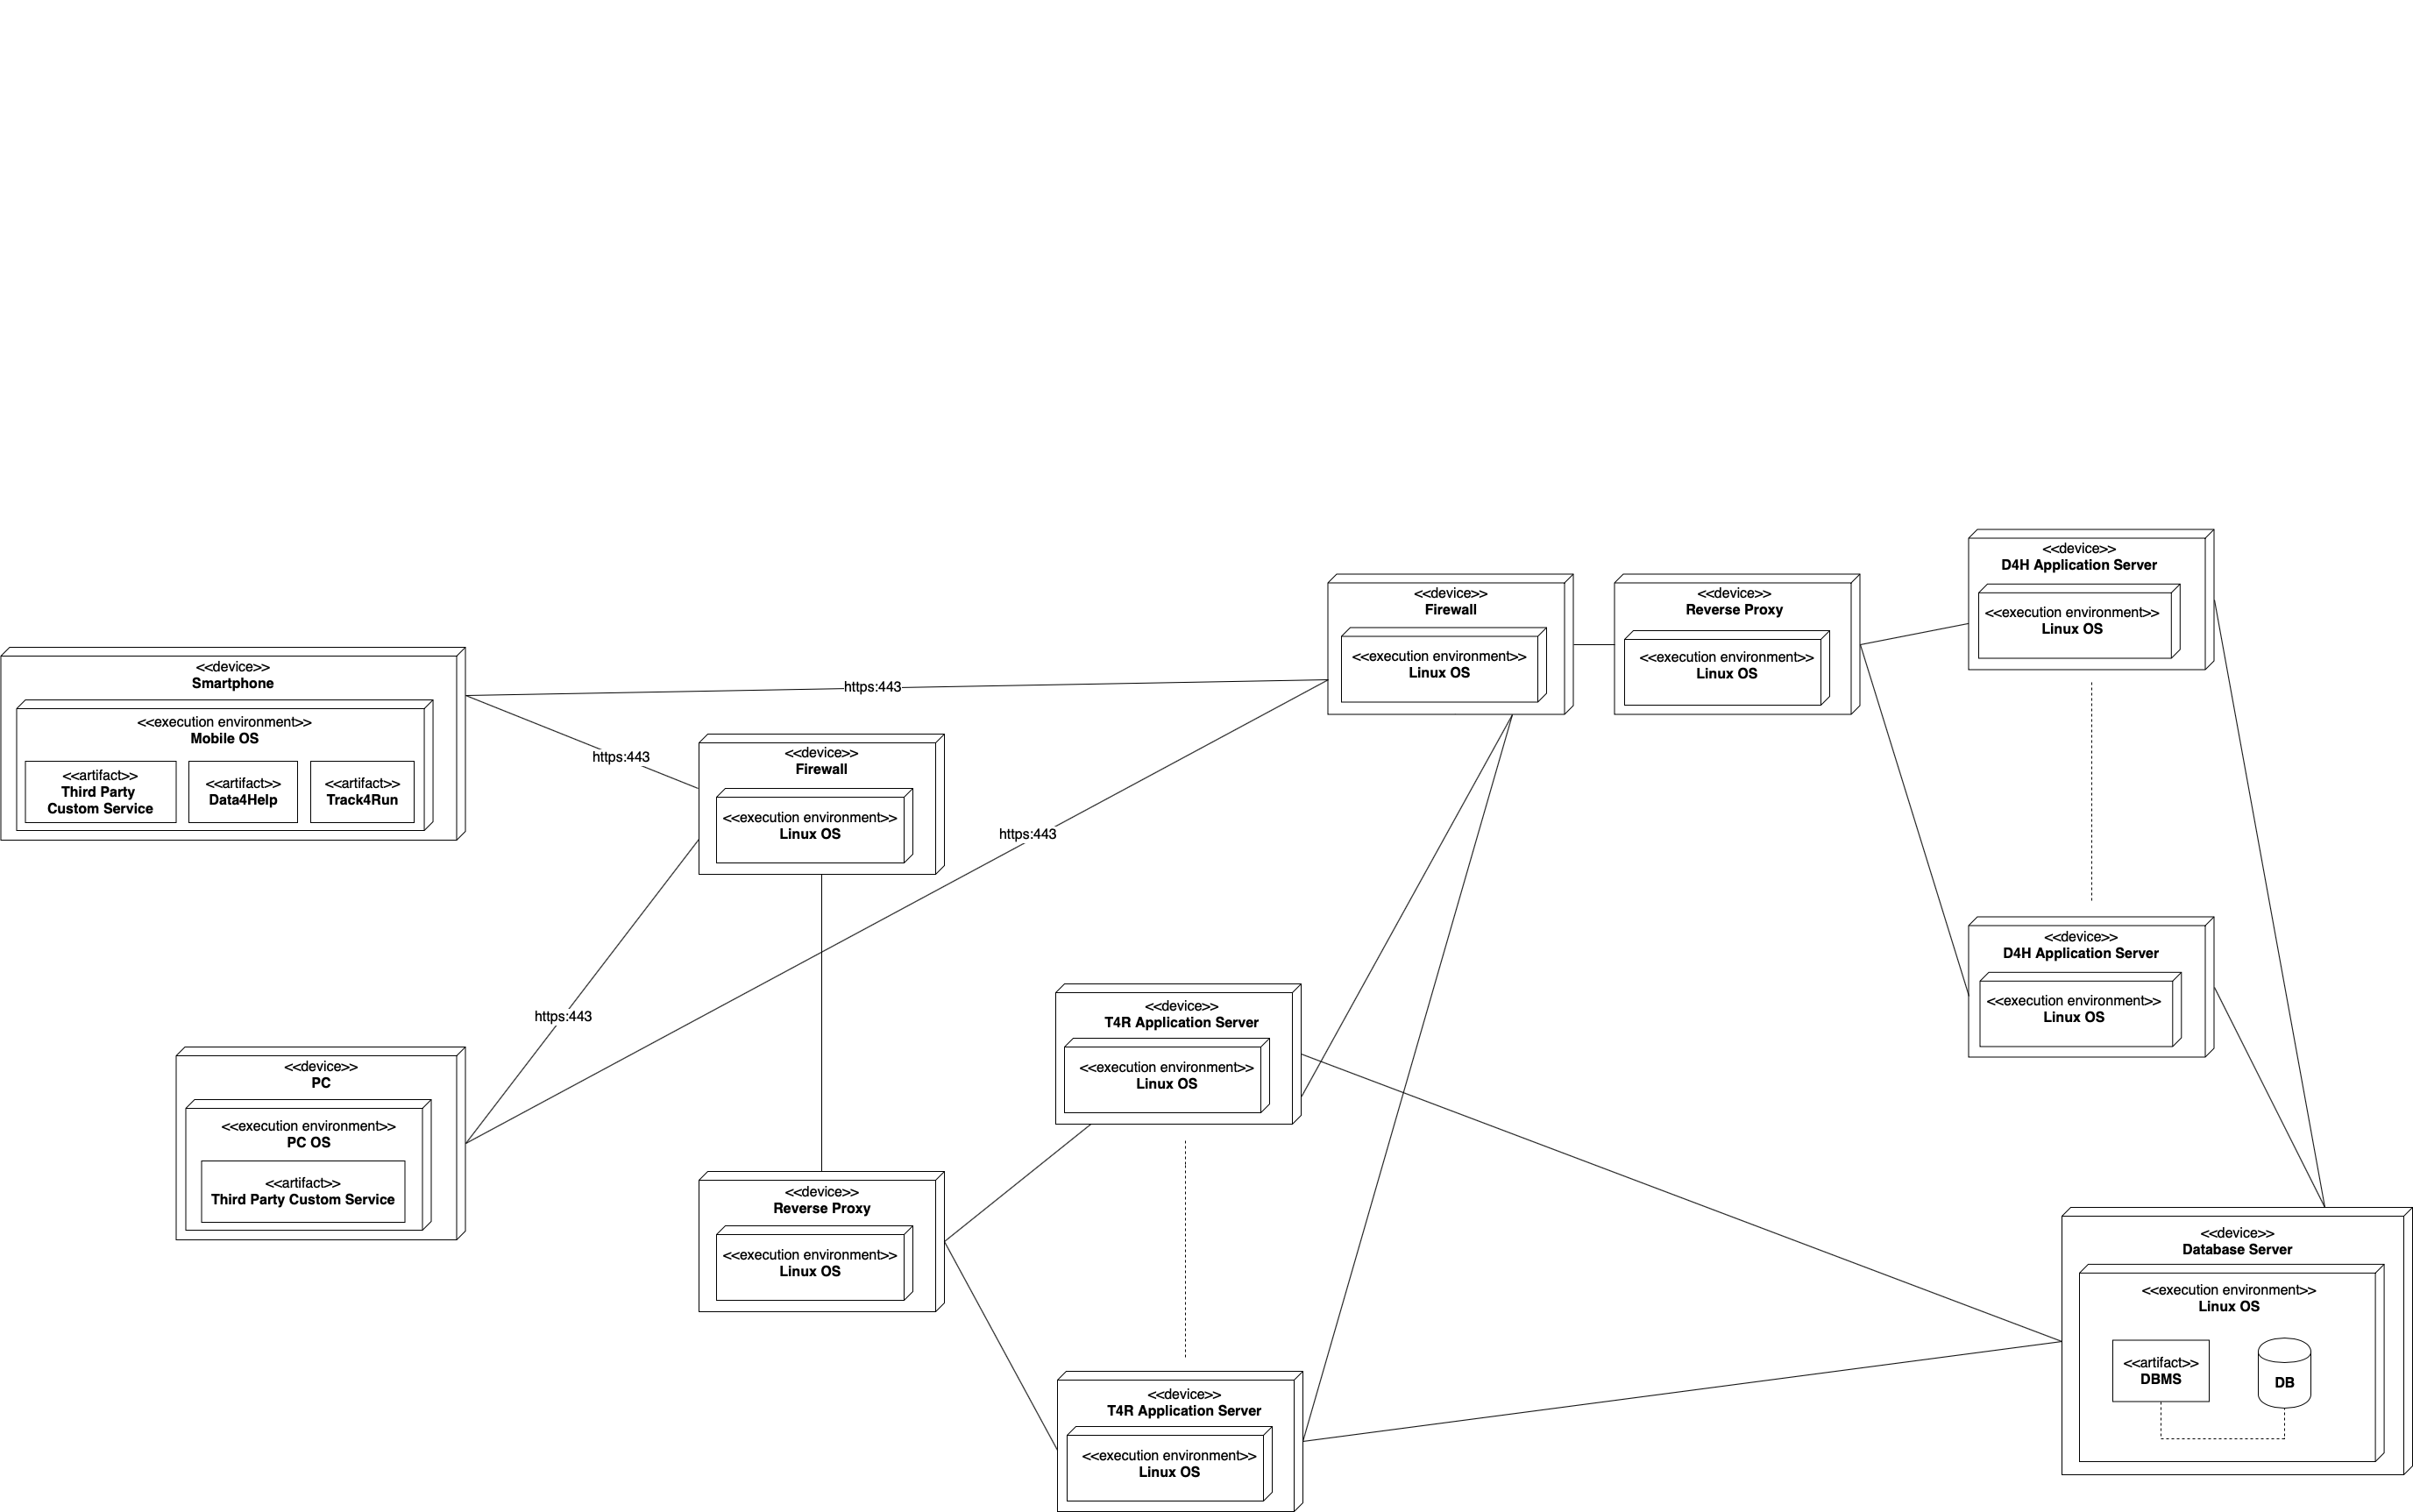
\includegraphics[width=10cm]{DeploymentView.png}
  	\caption{Deployment View}
 	\label{fig:DEPVIEW}
\end{figure}
The system presents a multi-tier architecture in which the role of each node will be specified in the next paragraphs. 

{\bf Smartphone }\\ 
This node acts as a client machine and could hosts Data4Help and Track4Run native applications. 

{\bf PC }\\ 
This node works as well as a client and grants third parties access to Data4Help functionalities through the use of a web browser.

{\bf Firewall }\\ 
This component filters the access to the Reverse Proxy and is used to protect a trusted network from an untrusted network. A firewall provides protection from unauthorized requests or from various types of malicious attacks like DDoS.

{\bf Application Servers }\\ 
This level of the architecture encloses all the business logic of the systems. Data4Help and Track4Run Application Servers are fully replicated to balance the workload. Track4Run Application Servers communicate with Data4Help ones in order to make use of their APIs.

{\bf Reverse Proxy }\\ 
This node helps to achieve increased parallelism and scalability. It is responsible for the load balancing as it distributes requests between all Application Servers. The Reverse Proxy also increases security and anonymity by protecting the identity of our backend servers and acting as an additional shield against security attacks.

{\bf Database Server }\\ 
This machine is equipped with a relational DBMS and it is used to store and retrieve all data needed by the Application Servers. 

\pagebreak


\subsection{Runtime view}

{\bf Proxy Runtime View }\\ 
The following sequence diagram describes how the Reverse Proxy, implemented using Nginx, interacts with the Client and the Application Server.
Whenever a Client forwards a request, the Reverse Proxy receives it on behalf of the Server, checks whether such request conforms to its defined schema and, in case the user has to be logged in, checks if the provided authToken is associated to an actual logged in user. This last check, in particular, is efficient to be done on the Proxy instead of each Application Server, because if a user logs in with a particular Server which then crashes, the user doesn’t have to log in again, since the information is stored on the Proxy. One alternative could be to save the information on the DB, but that would require a query for every request sent by the Client, since the interaction is stateless.
In all the diagrams following this one, the proxy will not be included for readability purposes, but keep in mind that it will analyze every request before forwarding it to the Server (but not checking the validity of the authToken when a user registers or spectates a run).

\begin{figure}[H]
	\center
  	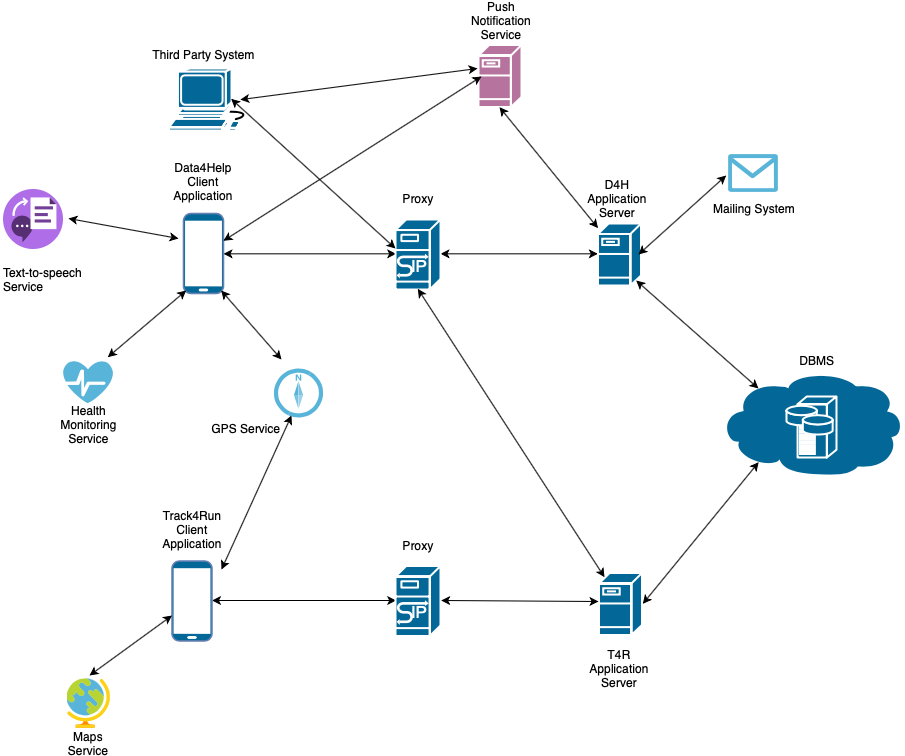
\includegraphics[width=10cm] {Overview.png}%{Proxy.png}
  	\caption{Proxy Runtime View}
 	\label{fig:PROXY}
\end{figure}


{\bf Registration Runtime View }\\ 
The following sequence diagram describes the order of events that occur whenever a user registers to Data4Help. The procedure is equivalent for both registering as a Single User and as a Third Party. The actors involved in this scenario are the Presentation and Network Manager components on the Client side and the Network Manager, Authentication Manager, Data Storage Manager on the Server Side. External services that are invoked are the DBMS and the Mailing System.
The sequence of events is guided by the user’s HTTP registration request, filled with the user’s email, password, FC, full name, birthdate and sex, all forming the “registration form”. The request is either malformed, such as having empty parameters, either structurally correct and defining the information to store in a new account in the database. However a request may still be invalid as it provides an already used email or FC, thus receiving an HTTP ERROR 403 response (Already Registered) or contains information violating the databases integrity constraints, thus receiving an HTTP ERROR 400 response (Malformed Request).
Finally, in order to activate a newly created account, a user will click on the URL provided in the confirmation email and this will automatically send and HTTP request of account activation. If the account has already been activated the user will receive an HTTP ERROR 403 (Already Activated). In the case of wrong tokens or malformed requests the user will receive either an HTTP ERROR 401(Wrong Token) or HTTP ERROR 400 response (Malformed Request).

\begin{figure}[H]
	\center
  	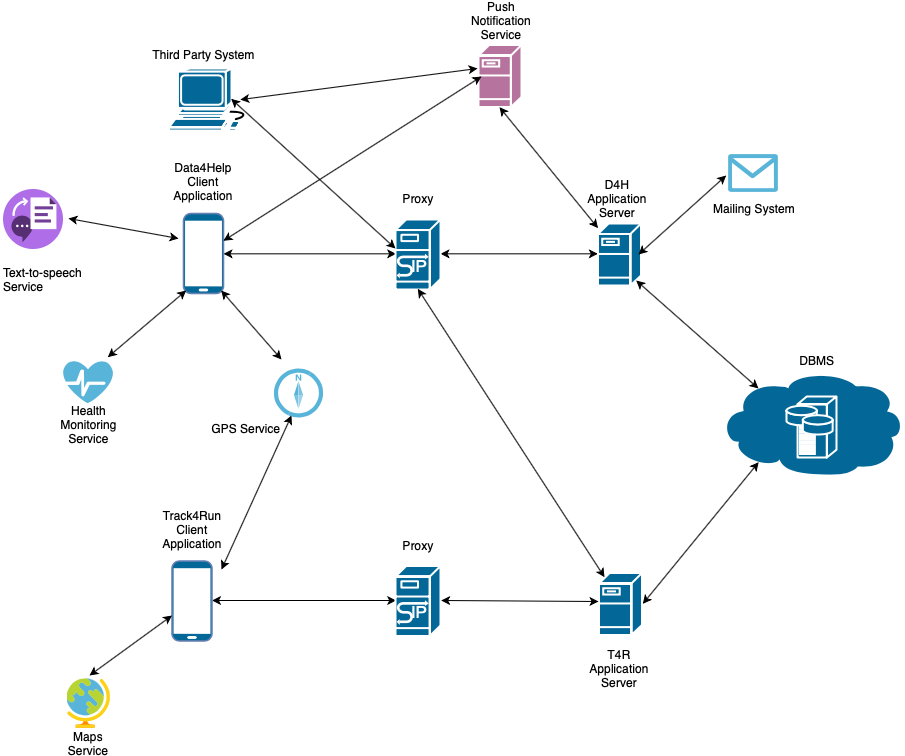
\includegraphics[width=10cm]{Overview.png} %{Registration.png}
  	\caption{Registration Runtime View}
 	\label{fig:REG}
\end{figure}


{\bf Login Runtime View }\\ 
The following diagram represents the sequence of events that occur when a user tries to log into his account, being either Single User or Third Party accounts. The actors involved in the scenario are the Presentation and Network Manager on the Client side and the Network Manager, Single User Manager and Data Storage Manager on the Server side. 
When a user logs into his account, an HTTP request is sent to the application server containing the user’s credentials. If the request’s format is invalid, such as having empty parameters, the user immediately receives an HTTP ERROR 400 (Malformed Request) response. If instead the request is structurally correct, the SIngle User Manager checks the validity of the credentials by querying the Database. If the credentials are wrong or malformed an HTTP ERROR 401 (Wrong Credentials) or HTTP ERROR 400 (Malformed Request) response are sent. If instead the user has already logged in with another device and is currently still logged he will receive an HTTP ERROR 403 (Already Logged-in) response.

\begin{figure}[H]
	\center
  	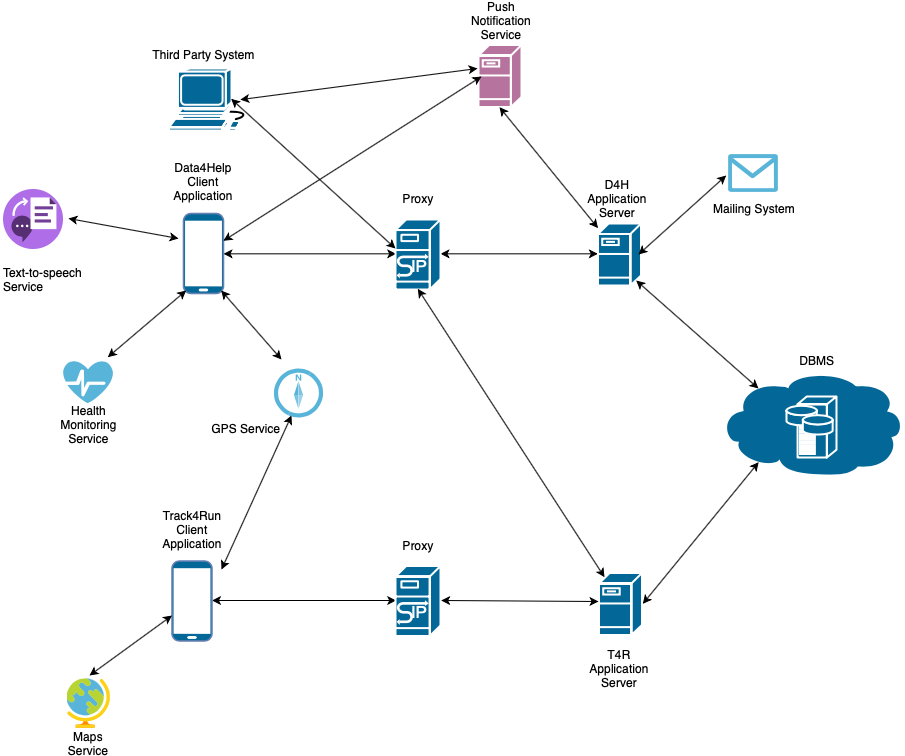
\includegraphics[width=10cm]{Overview.png} %{Login.png}
  	\caption{Login Runtime View}
 	\label{fig:LOG}
\end{figure}


{\bf Single Request Runtime View }\\ 
The following diagram describes the events that occur after a Single Request is sent by a Third Party to a Single User. There are many components involved in this interaction. On the Third Party and Single User client side the Presentation and the Network Manager. Server side there are the Network Manager, Single Request Manager and Data Storage Manager. Finally the DBMS is invoked as an external service.
When a Third Party select the research tab and enables all the parameters he is interested in, an HTTP request is sent to the Application server. A new Single Request is created by the Single Request Manager and it is stored into the database. After that a notification containing the data requested by the Third Party is sent to the appropriate Single User who can either decide to accept or decline it. If the request is declined a notification is sent to the Third Party and the status of the request in the DB is updated. If instead the request gets accepted, the Application Server with the help of the Single User Manager retrieves the requested data and send them to the Third Party.

\begin{figure}[H]
	\center
  	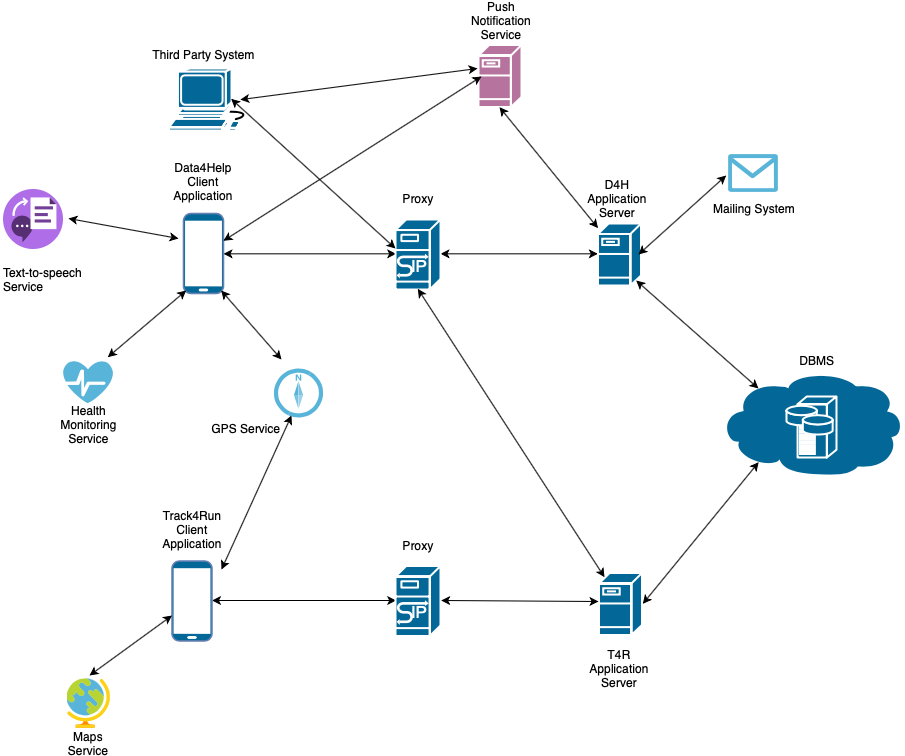
\includegraphics[width=10cm]{Overview.png} %{SingleRequest.png}
  	\caption{Single Request Runtime View}
 	\label{fig:SIGREQ}
\end{figure}


{\bf Group Request Runtime View }\\ 
The following diagram describes the events that occur after a Group Request is sent by a Third Party to Data4Help Application Server. The components involved in this interaction are the Third Party Presentation and Network Manager for client side and  on server side the Network Manager, Group Request Manager and Data Storage Manager. Finally the DBMS is invoked as an external service.
When a Third Party select the group research tab and selects all the parameters and filters he is interested in, an HTTP request is sent to the Application server. A new Group Request is created by the Group Request Manager and it is stored into the database. Then a query containing the parameters of the group request is sent to the DBMS. It retrieves the results and checks whether they are related to more than 1000 unique users. If not it sends back an empty response and the Group Request Manager with the help of the Network Manager notifies the Third Party that the request was not accepted. If the result matches more than 1000 unique users the Group Request Manager eventually enables the subscription option and sends the retrieved data to the Third Party.

\begin{figure}[H]
	\center
  	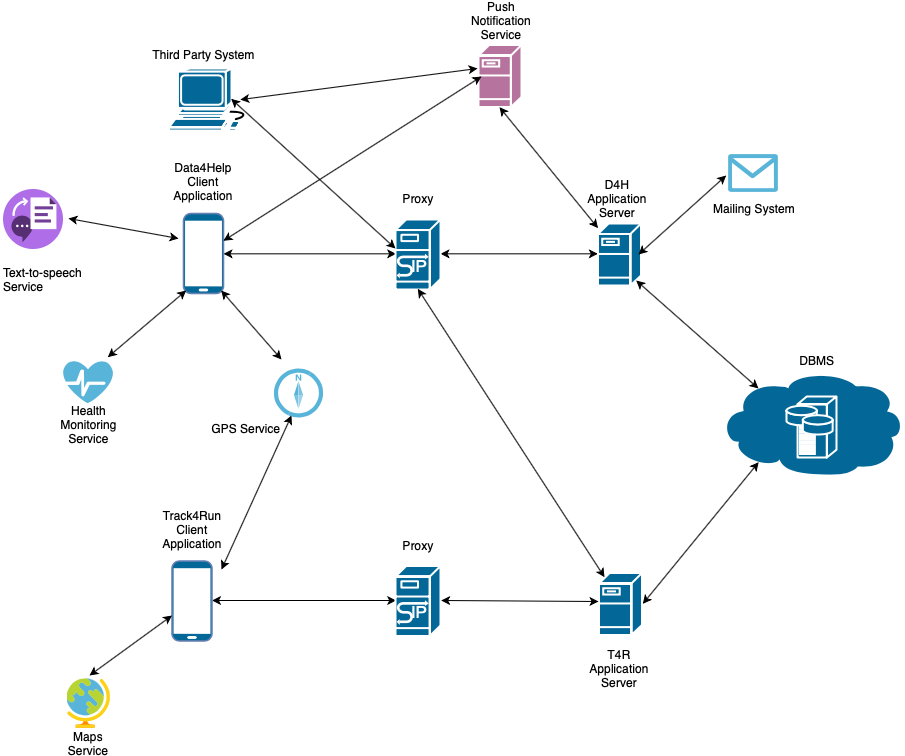
\includegraphics[width=10cm]{Overview.png} %{GroupRequest.png}
  	\caption{Group Request Runtime View}
 	\label{fig:GRPREQ}
\end{figure}


{\bf AutomatedSOS enabling Runtime View }\\ 
The following diagram represent the sequence of events that occurs when a Single User decides to enable automatedSOS and how said feature works.
The components involved are all part of the client side: Presentation, AutomatedSOS, GPS and TTS. A single User enable AutomatedSOS by pressing a toggle in MyHealth tab.
AutomatedSOS component is activated and start to periodically check the user health status. If parameters denoting a critical condition are observed, the current location of the subject is retrieved from the GPS module and AutomatedSOS converts a text message to speech, so it then performs an automated call to an ambulance.

\begin{figure}[H]
	\center
  	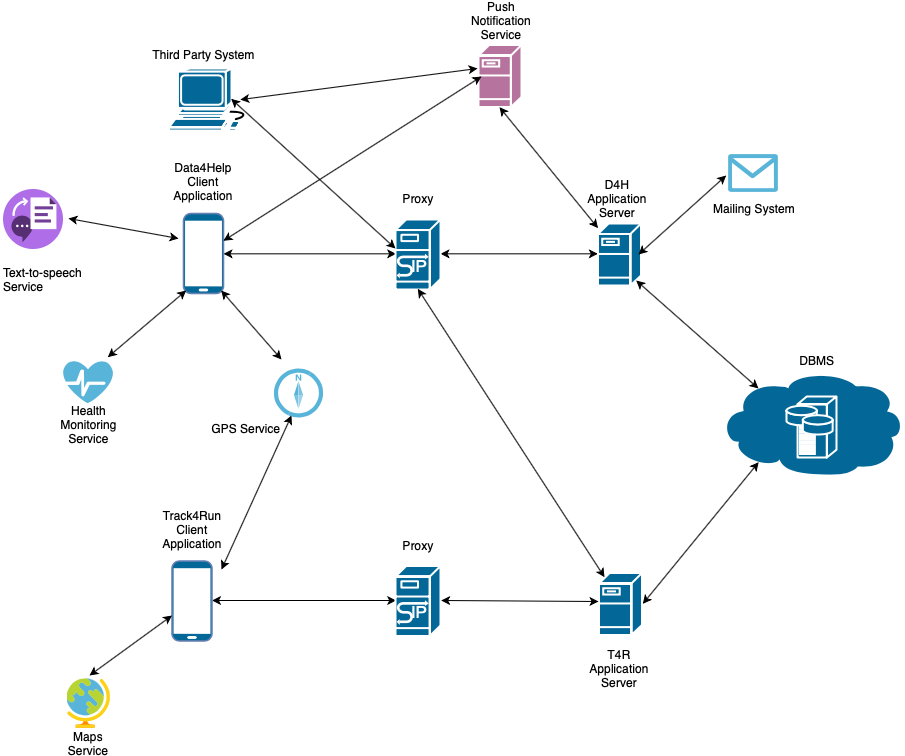
\includegraphics[width=10cm]{Overview.png} %{SOS.png}
  	\caption{AutomatedSOS enabling Runtime View}
 	\label{fig:SOS}
\end{figure}


{\bf Organize a Run Runtime View }\\ 
The following diagram describes the sequence of events that occur when a logged-in Third Party wants to create a run using Track4Run.
The components involved are the Third Party presentation and the Network Manager for the client, and the Network Manager, Run Manager and Data Storage Manager for the Application Server, who in turn interacts with the DB.
The sequence of events begins with the user opening the New Run tab on his mobile device, and providing as information the info of the run. The application server receives this data, updates the database and generates the RunID, which is then sent to the user. A path is defined by the user, but before checking its validity the server ensures that a correct RunID is provided. If so, the server proceeds to control that the path is feasible: if not it responds with a HTTP 401 Error message, otherwise it updates the DB and responds with a HTTP 200 OK message to the user, terminating the interaction.

\begin{figure}[H]
	\center
  	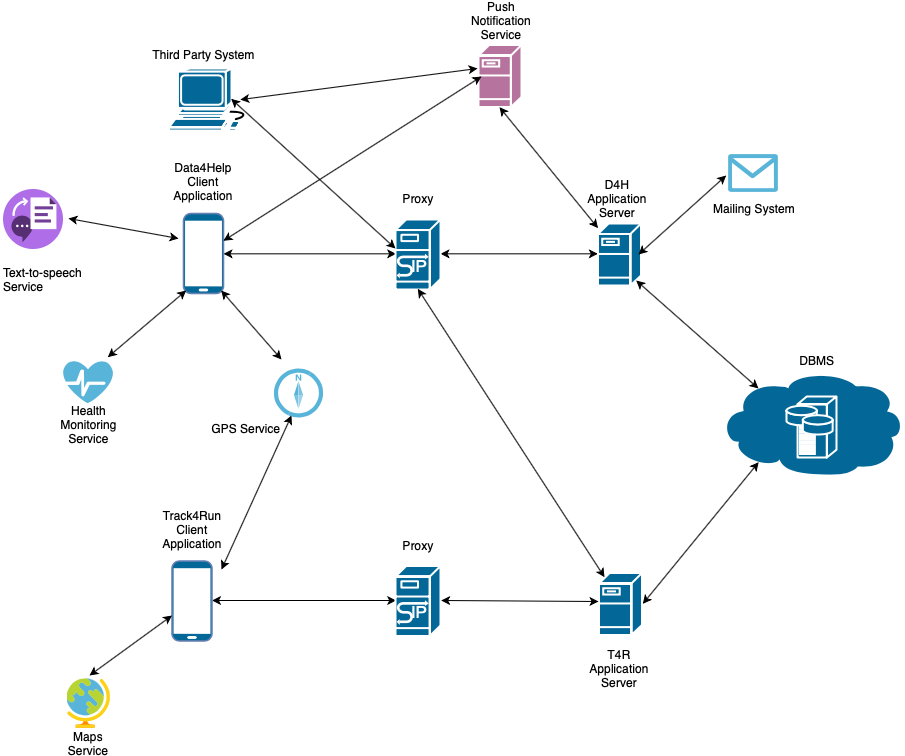
\includegraphics[width=10cm]{Overview.png} %{Organize.png}
  	\caption{Organize a Run Runtime View}
 	\label{fig:SOS}
\end{figure}


{\bf Join a Run Runtime View }\\ 
The following diagram describes the sequence of events that occur when a logged-in Private User wants to join a run using Track4Run.
The components involved are the Private User presentation and the Network Manager for the client, and the Network Manager, Active Runs Manager and Data Storage Manager for the Application Server, who in turn interacts with the DB.
The sequence of events begins with the user opening the Active Runs tab on his mobile device, sending a request to the server to obtain the list of active runs. The server responds with such list, and the user chooses an active run to join. If the run chosen is not valid, the server will respond with a HTTP 401 Error message, otherwise it will update the DB and list the user as a participant.
When the day of the run comes, the server pushes a request to Data4Help directly (avoiding the proxy as the user is already logged in Track4Run) which forwards it to every user, who has a timeout to accept it if he wants to take part in the run. If he doesn’t, he is removed from it, otherwise he’s listed as a definitive participant and the process terminates with a HTTP 200 OK message.

\begin{figure}[H]
	\center
  	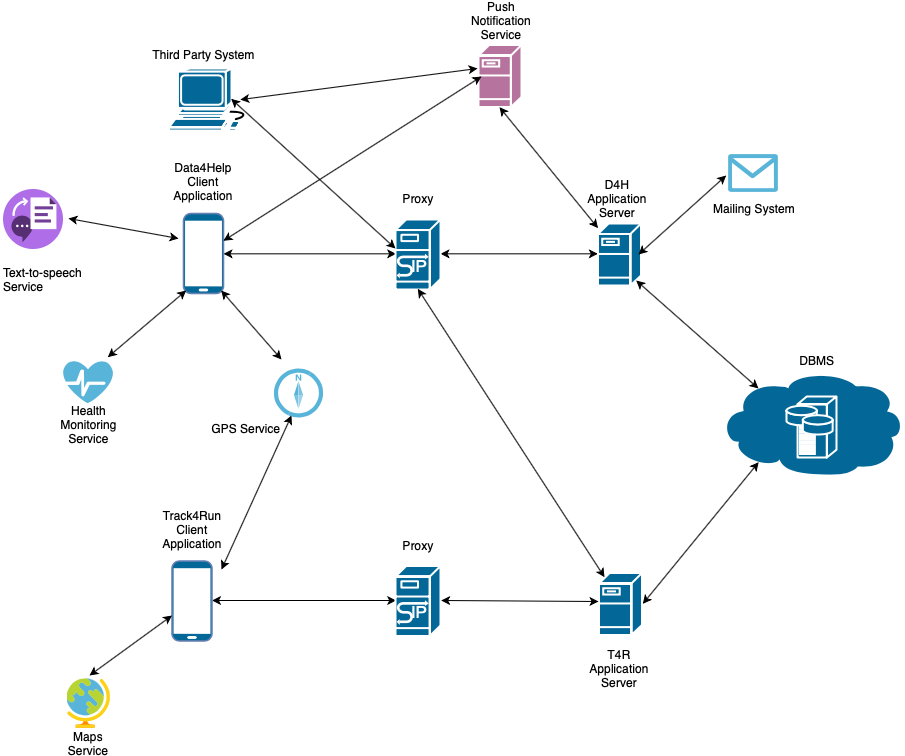
\includegraphics[width=10cm]{Overview.png} %{Join.png}
  	\caption{Join a Run Runtime View}
 	\label{fig:JOIN}
\end{figure}


{\bf Spectate a Run Runtime View }\\ 
The following diagram describes the sequence of events that occur whenever a user wants to spectate a run using Track4Run, without having to be logged in.
The components involved are the User presentation and the Network Manager for the client, and the Network Manager, Active Runs Manager and Data Storage Manager for the Application Server, who in turn interacts with the DB.
The sequence of events begins with the user opening the Active Runs tab on his mobile device, sending a request to the server to obtain the list of active runs. The server responds with such list and registers him as a spectator, then the user chooses an active run to spectate. If the run chosen is not valid, the server will respond with a HTTP 401 Error message, otherwise it will update the DB and list the user as a spectator for that run. The process terminates with a HTTP 200 OK message, allowing the user to watch the run live on his device.

\begin{figure}[H]
	\center
  	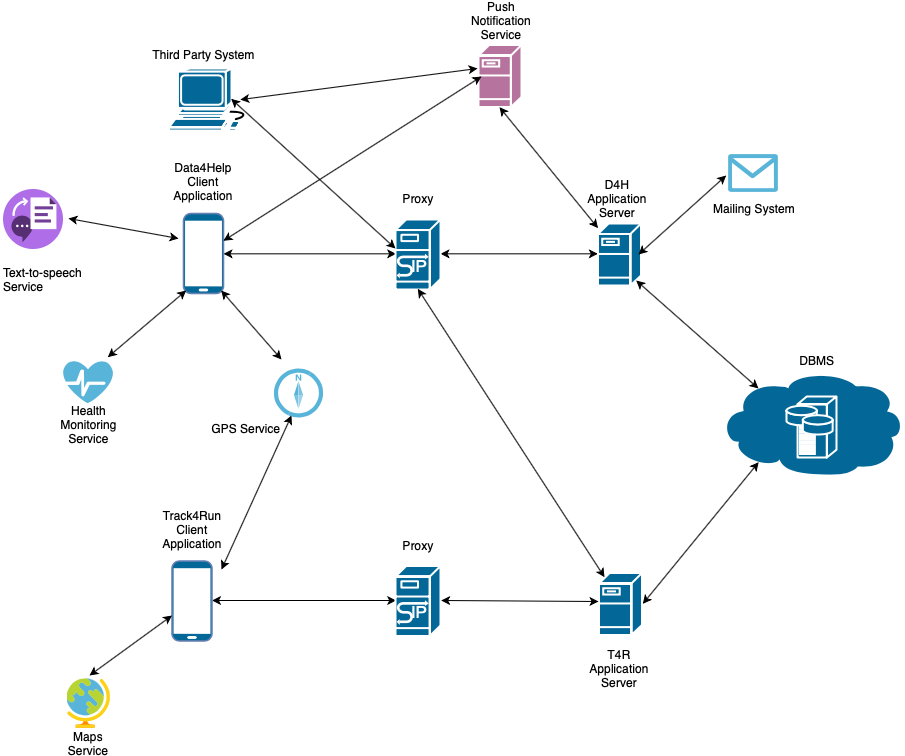
\includegraphics[width=10cm]{Overview.png} %{Spectate.png}
  	\caption{Spectate a Run Runtime View}
 	\label{fig:SPEC}
\end{figure}

\pagebreak



\subsection{Component interfaces}

{\bf Interface Diagram }\\ 
Please note that, for readability purposes, most methods requiring the authentication token identifying a specific user do not take it as input parameter.
Also, all methods shown in the Runtime Views that are self-calls are obviously not included here, as they are not exposed to the outside through an interface

\begin{figure}[H]
	\center
  	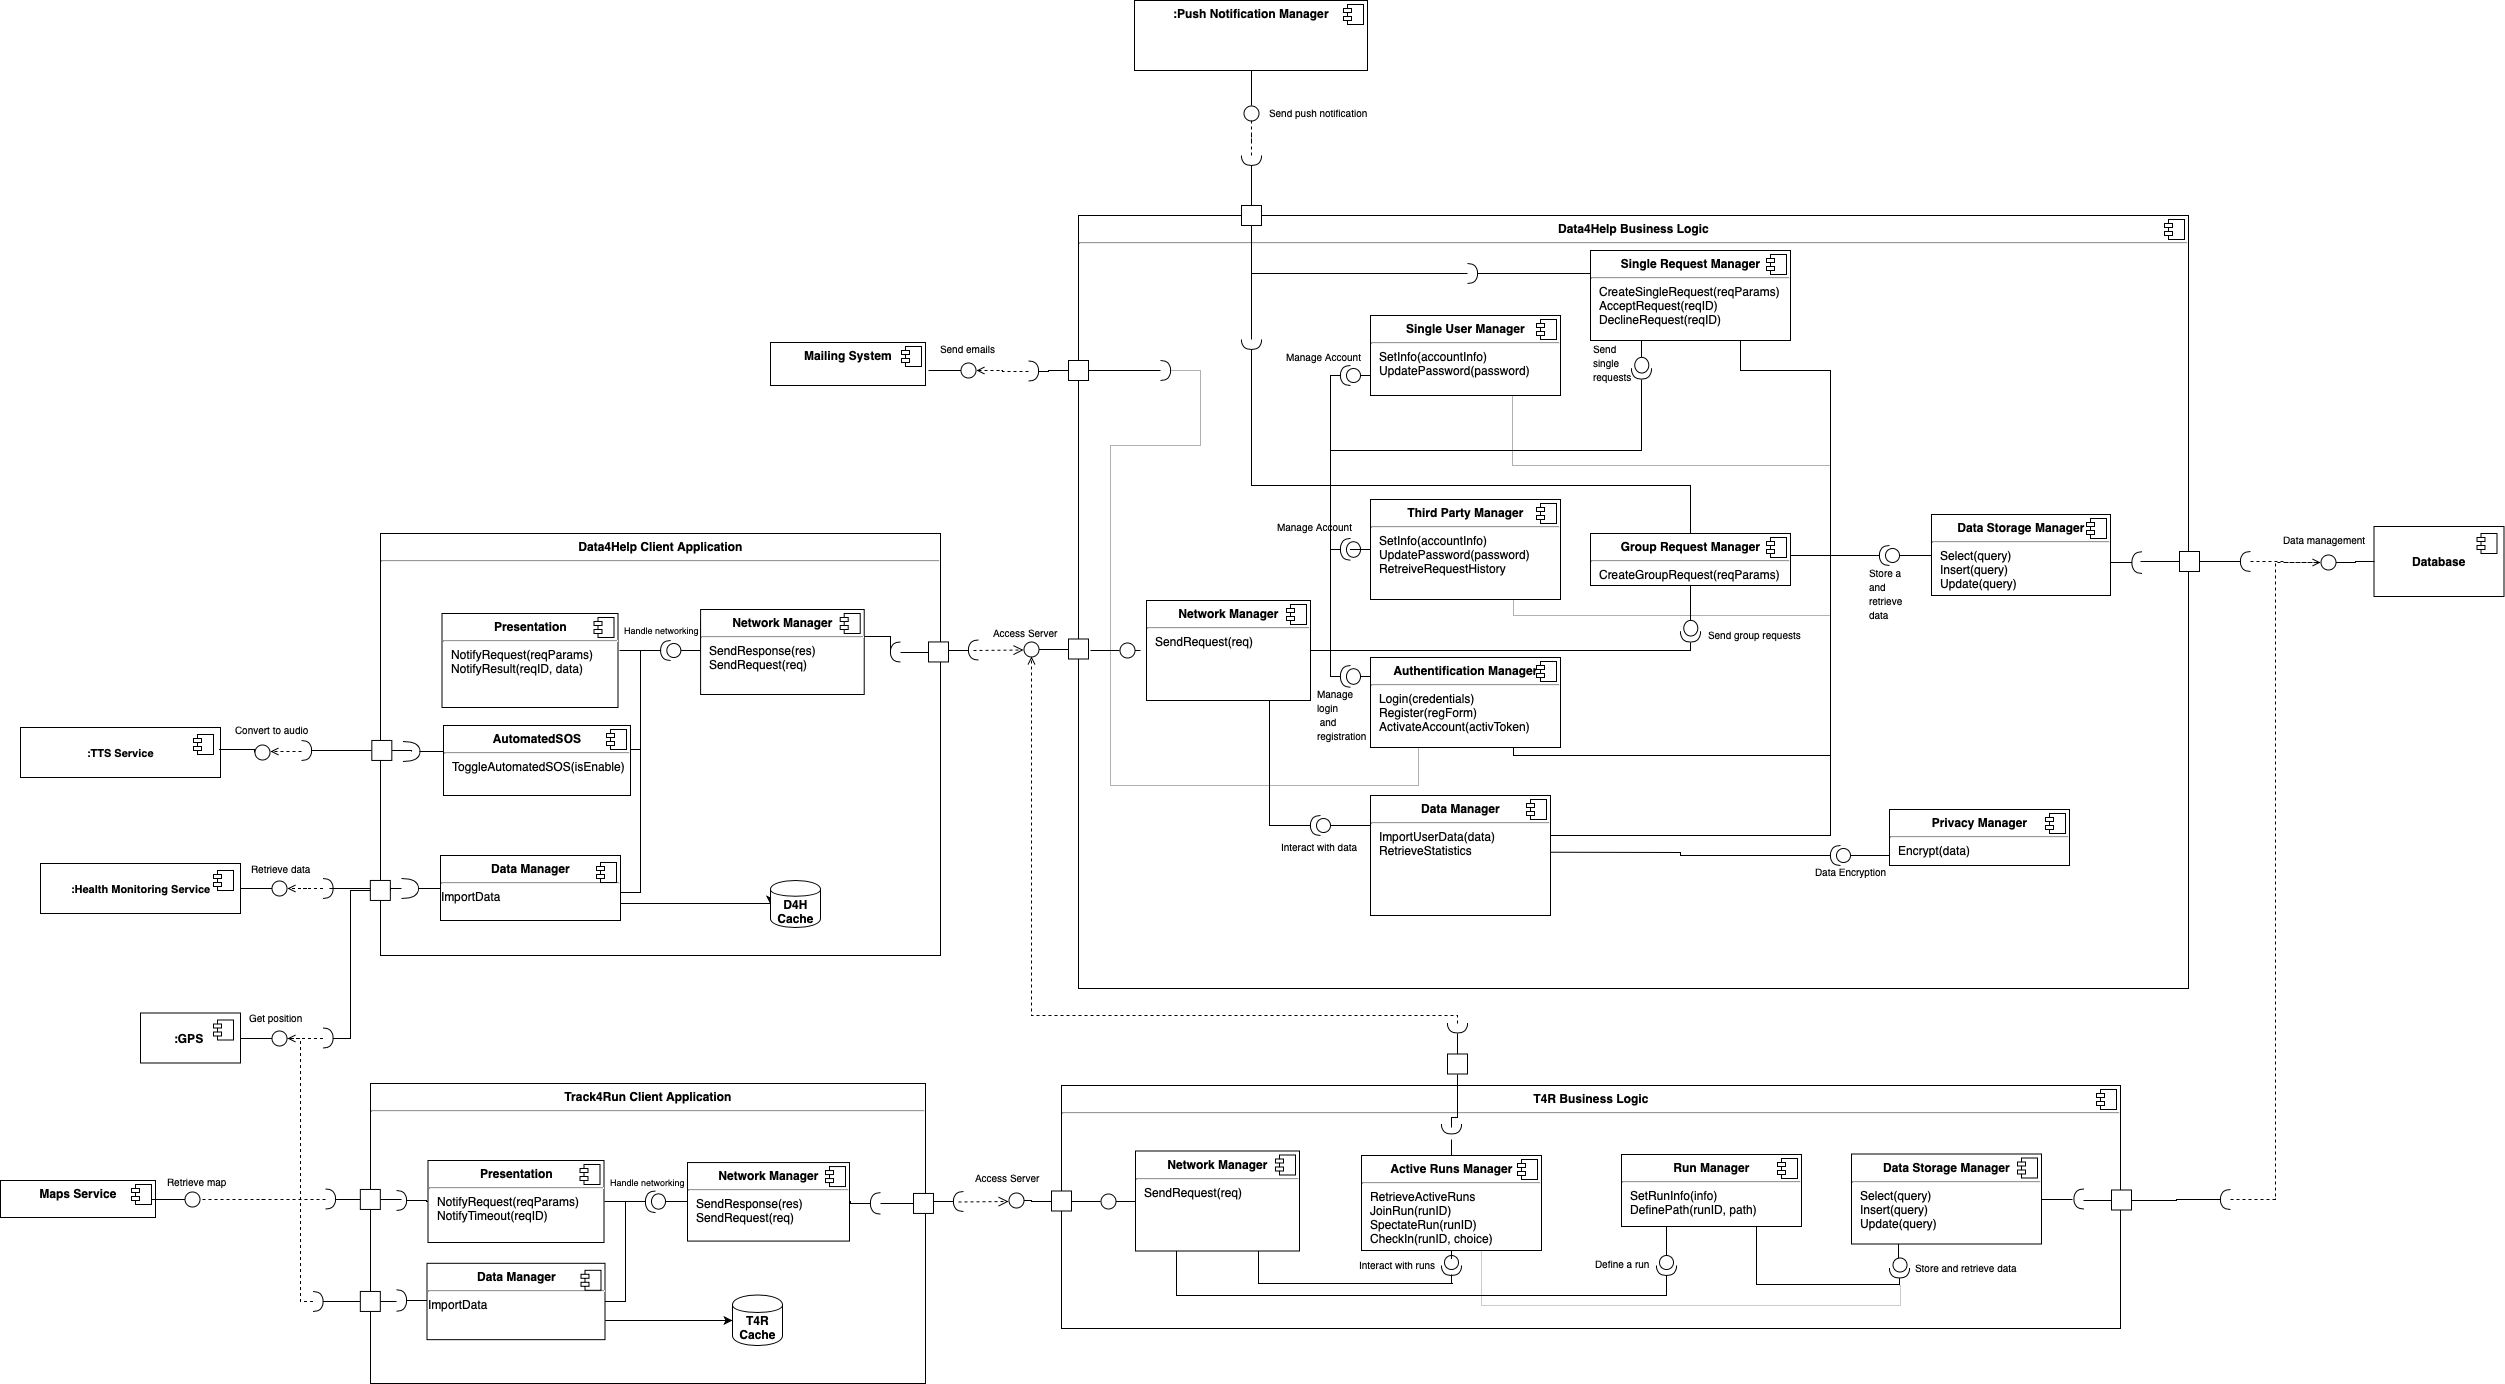
\includegraphics[width=10cm]{ComponentInterfaces.png}
  	\caption{Component interface diagram}
 	\label{fig:INT}
\end{figure}

\pagebreak

{\bf REST API}

\begin{tabularx}{\textwidth}{lX} \hline
    info & Lets single users register to the service \\ \hline
    endpoint & /*auth/reg/single \\ \hline
    type & POST \\ \hline
    req schema & 
        email : [string] \newline
        password : [string] \newline
        fc : [string] \newline
        full\_name : [string] \newline
        birthdate : [date] \newline
        sex : [string] \\ \hline
    success code &
        code: 200 OK \newline 
        body : \{ \newline
        "message" : "Registration successful" \newline
        \} \\ \hline
    error code &
        code: 400 \newline
        body : \{ "error" : "Malformed request" \} \newline \newline
        code: 403 \newline
        body : \{ "error" : "Already registered" \}  \\ \hline
\end{tabularx}

\vspace{\baselineskip}

\begin{tabularx}{\textwidth}{lX} \hline
    info & Lets third parties register to the service \\ \hline
    endpoint & /*auth/reg/tp \\ \hline
    type & POST \\ \hline
    req schema & 
        email : [string] \newline
        password : [string] \newline
        piva : [string] \newline
        company\_name : [string] \newline
        company\_description : [string] \\ \hline
    success code &
        code: 200 OK \newline \newline 
        body : \{ \newline
        "message" : "Registration successful" \newline
        \} \\ \hline
    error code &
        code: 400 \newline
        body : \{ "error" : "Malformed request" \} \newline \newline
        code: 403 \newline
        body : \{ "error" : "Already registered" \} \\ \hline
\end{tabularx}
		
\vspace{\baselineskip}

\begin{tabularx}{\textwidth}{lX} \hline
    info & Lets a user log in the service \\ \hline
    endpoint & /*auth/login \\ \hline
    type & POST \\ \hline
    req schema & 
        email : [string] \newline
        password : [string] \\ \hline
    success code &
        code: 200 OK \newline \newline 
        body : \{ \newline
        "message" : "Registration successful" \newline
        "authToken" : [string] \newline
        \} \\ \hline
    error code &
        code: 400 \newline
        body : \{ "error" : "Malformed request" \} \newline \newline
        code: 401 \newline
        body : \{ "error" : "Wrong credentials" \} \newline \newline
        code: 403 \newline
        body : \{ "error" : "Already logged in" \} \\ \hline
\end{tabularx}
		
\vspace{\baselineskip}

\begin{tabularx}{\textwidth}{lX} \hline
    info & Lets a user activate its account \\ \hline
    endpoint & */auth/activ?activToken=[string] \\ \hline
    type & GET \\ \hline
    req schema & \\ \hline
    success code &
        code: 200 OK \newline \newline 
        body : \{ \newline
        "message" : "Account activated" \newline
        \} \\ \hline
    error code &
        code: 401 \newline
        body : \{ "error" : "Wrong token" \} \newline \newline
        code: 403 \newline
        body : \{ "error" : "Already activated" \} \\ \hline
\end{tabularx}
		
\vspace{\baselineskip}

\begin{tabularx}{\textwidth}{lX} \hline
    info & Lets a private user modify his account info \\ \hline
    endpoint & */settings/single/info \\ \hline
    type & POST \\ \hline
    req schema & 
        authToken : [string] \newline
        password : [string] \newline
        full\_name : [string] \newline
        birthdate : [date] \newline
        sex : [string] \\ \hline
    success code &
        code: 200 OK \newline \newline 
        body : \{ \newline
        "message" : "Settings updated" \newline
        \} \\ \hline
    error code &
        code: 400 \newline
        body : \{ "error" : "Malformed request" \} \newline \newline
        code: 403 \newline
        body : \{ "error" : "Wrong token" \} \\ \hline
\end{tabularx}
		
\vspace{\baselineskip}

\begin{tabularx}{\textwidth}{lX} \hline
    info & Lets a private user modify his importable data \\ \hline
    endpoint & */settings/single/data \\ \hline
    type & POST \\ \hline
    req schema & 
        authToken : [string] \newline
        types : [[boolean]] \\ \hline
    success code &
        code: 200 OK \newline \newline 
        body : \{ \newline
        "message" : "Settings updated" \newline
        \} \\ \hline
    error code &
        code: 400 \newline
        body : \{ "error" : "Malformed request" \} \newline \newline
        code: 403 \newline
        body : \{ "error" : "Wrong token" \} \\ \hline
\end{tabularx}
		
\vspace{\baselineskip}

\begin{tabularx}{\textwidth}{lX} \hline
    info & Lets a third party user modify his account info \\ \hline
    endpoint & */settings/tp/info \\ \hline
    type & POST \\ \hline
    req schema & 
    "authToken": [string] \newline
    "company name": [string] \newline
    "company description": [string] \newline
    "password": [string] \\ \hline
    success code &
        code: 200 OK \newline \newline 
        body : \{ \newline
        "message" : "Settings updated" \newline
        \} \\ \hline
    error code &
        code: 400 \newline
        body : \{ "error" : "Malformed request" \} \newline \newline
        code: 403 \newline
        body : \{ "error" : "Wrong parameters" \} \\ \hline
\end{tabularx}
		
\vspace{\baselineskip}

\begin{tabularx}{\textwidth}{lX} \hline
    info & Lets a private user retrieve a list of all requests meant for him \\ \hline
    endpoint & */req/single/list?authToken=[string] \\ \hline
    type & GET \\ \hline
    req schema & \\ \hline
    success code & body: \{ \newline
    "requests": [ \newline
    \{ \newline
    "reqID": [string] \newline
    "email": [string] \newline
    "piva": [string] \newline
    "company name": [string] \newline
    "dataTypes": [[string],...[string]] \newline
    "status": [string] \newline
    "subscribing": [bool] \newline
    "duration": [int] \newline
    \} \newline
    ] \newline
    \} \\ \hline
    error code &
        code: 400 \newline
        body : \{ "error" : "Malformed request" \} \newline \newline
        code: 403 \newline
        body : \{ "error" : "Wrong token" \} \\ \hline
\end{tabularx}
		
\vspace{\baselineskip}

\begin{tabularx}{\textwidth}{lX} \hline
    info & Lets a third party retrieve the list of its requests \\ \hline
    endpoint & */req/tp/list?authToken=[string] \\ \hline
    type & GET \\ \hline
    req schema & \\ \hline
    success code & body: \{ \newline
    "requests": [ \newline
    \{ \newline
    "reqID": [string] \newline
    "email": [string] \newline
    "fc": [string] \newline
    "dataTypes": [[string],...[string]] \newline
    "searchParams": [[string],...[string]] \newline
    "status": [string] \newline
    "subscribing": [bool] \newline
    "duration": [int] \newline
    \} \newline
    ] \newline
    \} \\ \hline
    error code &
        code: 400 \newline
        body : \{ "error" : "Malformed request" \} \newline \newline
        code: 403 \newline
        body : \{ "error" : "Wrong parameters" \}\\ \hline
\end{tabularx}
		
\vspace{\baselineskip}

\begin{tabularx}{\textwidth}{lX} \hline
    info & Lets a third party send a single request \\ \hline
    endpoint & */req/tp/sendSingle \\ \hline
    type & POST \\ \hline
    req schema & 
    "authToken": [string] \newline
    "reqID": [string] \newline
    "email": [string] \newline
    "fc": [string] \newline
    "dataTypes": [[string],...[string]] \newline
    "subscribing": [bool] \newline
    "duration": [int] \\ \hline
    success code &
        code: 200 OK \newline \newline 
        body : \{ \newline
        "reqID" : [string] \newline
        \} \\ \hline
    error code &
        code: 400 \newline
        body : \{ "error" : "Malformed request" \} \newline \newline
        code: 401 \newline
        body : \{ "error" : "Wrong parameters" \}\\ \hline
\end{tabularx}
		
\vspace{\baselineskip}

\begin{tabularx}{\textwidth}{lX} \hline
    info & Lets a third party send a group request \\ \hline
    endpoint & */req/tp/sendGroup \\ \hline
    type & POST \\ \hline
    req schema &
    "authToken": [string] \newline
    "reqID": [string] \newline
    "dataTypes": [[string],...[string]] \newline
    "searchParams": [[string],...[string]] \newline
    "subscribing": [bool] \newline
    "duration": [int] \\ \hline
    success code &
        code: 200 OK \newline \newline 
        body : \{ \newline
        "reqID" : [string] \newline
        \} \\ \hline
    error code &
        code: 400 \newline
        body : \{ "error" : "Malformed request" \} \newline \newline
        code: 403 \newline
        body : \{ "error" : "Wrong parameters" \}\\ \hline
\end{tabularx}
		
\vspace{\baselineskip}

\begin{tabularx}{\textwidth}{lX} \hline
    info & Lets a private user accept or decline a single request \\ \hline
    endpoint & */req/single/choice \\ \hline
    type & POST \\ \hline
    req schema & 
    "authToken": [string] \newline
    "reqID": [string] \newline
    "choice": [string] \\ \hline
    success code &
        code: 200 OK \newline \newline 
        body : \{ \newline
        "message" : "Action successful" \newline
        \} \\ \hline
    error code &
        code: 400 \newline
        body : \{ "error" : "Malformed request" \} \newline \newline
        code: 403 \newline
        body : \{ "error" : "Wrong parameters" \}\\ \hline
\end{tabularx}
		
\vspace{\baselineskip}

\begin{tabularx}{\textwidth}{lX} \hline
    info & Lets a private user load data \\ \hline
    endpoint & */data/upload \\ \hline
    type & POST \\ \hline
    req schema & 
    "authToken": [string] \newline
    "dataTypes": [[string],...[string]] \newline
    "values": [[string],...[string]] \newline
    "timestamp": [[string],...[string]] \\ \hline
    success code &
        code: 200 OK \newline \newline 
        body : \{ \newline
        "message" : "Action successful" \newline
        \} \\ \hline
    error code &
        code: 400 \newline
        body : \{ "error" : "Malformed request" \} \newline \newline
        code: 403 \newline
        body : \{ "error" : "Wrong parameters" \}\\ \hline
\end{tabularx}
		
\vspace{\baselineskip}

\begin{tabularx}{\textwidth}{lX} \hline
    info & Lets a private user retrieve statistics \\ \hline
    endpoint & */data/stats?authToken=[string] \\ \hline
    type & GET \\ \hline
    req schema & 
        email : [string] \newline
        password : [string] \\ \hline
    success code &
        code: 200 OK \newline \newline 
        "body" : \{ \newline
        "dataTypes" : [\newline
        \{
        "parameter": [string] \newline
        "median": [int] \newline
        "date": [int] \newline
        \}
        ] \newline
        \} \\ \hline
    error code &
        code: 400 \newline
        "body" : \{ "error" : "Malformed request" \} \newline \newline
        code: 403 \newline
        "body" : \{ "error" : "Wrong parameters" \} \\ \hline
\end{tabularx}
		
\vspace{\baselineskip}

\begin{tabularx}{\textwidth}{lX} \hline
    info & Lets a third party create a run \\ \hline
    endpoint & */t4r/org/create \\ \hline
    type & POST \\ \hline
    req schema &  \newline
    "authToken": [string] \newline
    "runName": [string] \newline
    "startTime": [string] \newline
    "endTime": [string] \newline
    "participants": [int] \\ \hline
    success code &
        code: 200 OK \newline \newline 
        "body" : \{ \newline
        "message" : "Info set successfully" \newline
        "runID" : [int] \newline
        \} \\ \hline
    error code &
        code: 400 \newline
        "body" : \{ "error" : "Malformed request" \} \newline \newline
        code: 401 \newline
        "body" : \{ "error" : "Wrong credentials" \} \\ \hline
\end{tabularx}
		
\vspace{\baselineskip}

\begin{tabularx}{\textwidth}{lX} \hline
    info & Lets a third party set the path for a run \\ \hline
    endpoint & */t4r/org/path \\ \hline
    type & POST \\ \hline
    req schema & 
        "authToken": [string] \newline
        "runID": [int] \newline
        "path" : [ \newline
        \{ \newline
        "coordinate" : [string] \newline
        \} \newline
        ]
        \\ \hline
    success code &
        code: 200 OK \newline \newline 
        "body" : \{ \newline
        "message" : "Run created successfully" \newline
        \} \\ \hline
    error code &
        code: 400 \newline
        "body" : \{ "error" : "Malformed request" \} \newline \newline
        code: 401 \newline
        "body" : \{ "error" : "Invalid path" \} \newline \newline
        code: 401 \newline
        "body" : \{ "error" : "Wrong credentials" \} \newline \newline
        code: 401 \newline
        "body" : \{ "error" : "Wrong runID" \} \\\hline
\end{tabularx}
		
\vspace{\baselineskip}

\begin{tabularx}{\textwidth}{lX} \hline
    info & Lets a user (not necessarily logged in) fetch a list of active runs \\ \hline
    endpoint & */t4r/active/list \\ \hline
    type & GET \\ \hline
    req schema & \\ \hline
    success code &
        code: 200 OK \newline \newline 
        "body" : \{ \newline
        "run" : [ \{ \newline
        "runID": [string] \newline
        "runName": [string] \newline
        "startTime": [string] \newline
        "endPoint": [string] \newline
        "participants": [int] \newline
        \} ] \newline
        \} \\ \hline
    error code & \\ \hline
\end{tabularx}
		
\vspace{\baselineskip}

\begin{tabularx}{\textwidth}{lX} \hline
    info & Lets a private user join an active run \\ \hline
    endpoint & */t4r/active/join \\ \hline
    type & POST \\ \hline
    req schema & \newline
    "authToken": [string] \newline
    "runID": [int] \\ \hline
    success code &
        code: 200 OK \newline  
        "body" : \{ \newline
        "message" : "Run joined successfully" \newline
        \} \\ \hline
    error code &
        code: 400 \newline
        "body" : \{ "error" : "Malformed request" \} \newline \newline
        code: 401 \newline
        "body" : \{ "error" : "Wrong runID" \} \newline \newline
        code: 401 \newline
        "body" : \{ "error" : "Wrong credentials" \} \\ \hline
\end{tabularx}
		
\vspace{\baselineskip}

\begin{tabularx}{\textwidth}{lX} \hline
    info & Lets a spectator choose a active run \\ \hline
    endpoint & */t4r/active/spec \\ \hline
    type & POST \\ \hline
    req schema & “runID” : [int] \\ \hline
    success code &
        code: 200 OK \newline \newline 
        "body" : \{ \newline
        "path" : [ \newline
        \{ \newline
        "coordinate": [string] \newline
        \} \newline
        \} \\ \hline
    error code &
        code: 401 \newline
        "body" : \{ "error" : "Wrong runID" \} \\ \hline 
\end{tabularx}
		
\vspace{\baselineskip}

\begin{tabularx}{\textwidth}{lX} \hline
    info & Lets a spectator get the coordinates of runners \\ \hline
    endpoint & */t4r/active/specUpdate \\ \hline
    type & POST \\ \hline
    req schema & 
        “runID” : [int] \\ \hline
    success code &
        code: 200 OK \newline  
        "body" : \{ \newline
        [ \newline
        “runnerName” : [string] \newline
        “coordinate” : [string] \newline
        ] \newline
        \} \\ \hline
    error code &
        code: 401 \newline
        "body" : \{ "error" : "Wrong runID" \} \\ \hline
\end{tabularx}
		
\vspace{\baselineskip}

\pagebreak



\subsection{Selected architectural styles and patterns}

{\bf Multi-tier Architecture }\\ 
As stated in the Overview, the chosen architecture for the System is a multi-tier architecture, with three partially distributed layers. This division guarantees that each tier only deals with a specific task, so that computation is correctly spread amongst the System and there isn’t a central node in charge of everything. Also, modifications to a specific layer won’t affect the others, so the overall maintenance of the System is much easier.\\

In the first tier there is the Client’s physical device, which can be a mobile device or a desktop PC, in the case of Third Parties directly accessing the Application Server.
The Presentation layer is completely managed by this tier, with the aim of displaying to the user all informations received by the Application Server. This is done through a dynamic GUI on the mobile device, which also displays services offered by third parties such as the Map visualization service, used by Track4Run. Desktop PCs, on the other hand, do not implement the Presentation layer, as their only use of Data4Help and Track4Run is to query their APIs inside specific environments defined by the users.
Mobile devices also implement part of the business logic to guarantee the fulfillment of AutomatedSOS's nonfunctional requirements, and part of the data storage, as they hold a cache for data collected in the last week. Since these contributions to the Business and Data Storage layer are minimal, we will consider the Client tier to only implement the Presentation layer, thus being a Thin Client.\\

In the second tier there is have the Nginx Web Server, functioning both as a reverse proxy and as a load balancer. The purposes of these machines, used by Data4Help and Track4Run, is:
To retrieve data from the Application Servers and provide it to the Client as if the proxy were the server itself.
To redirect requests to the idle servers, avoiding congestions on each one.
Nginx was chosen over Apache for its flexibility in handling requests and its efficient use of main memory, thanks to the event-driven approach used.
This tier contributes to the implementation of the Business Logic layer, even though it doesn’t do it directly, but it helps the Application Servers in doing it.\\

In the third tier there is the Application Servers of Data4Help and Track4Run. The deployment will be done by replicating each server no more than three times, as initially the load will be low, and in case of a sudden increase we could seamlessly add more machines to handle the traffic, as each one is stateless. In fact, this tier only implements the Business and Domain Logic layer, but not the Data Storage layer. \\

In the fourth and final tier we have the Database, shared by Data4Help and Track4Run. This tier is not handled by TrackMe directly, as a cloud solution was preferred to one on premises, sparing the company from having to ensure the reliability of the DB and its management. 
This tier fully implements the Data Storage layer.\\

{\bf REST}\\
The Representational State Transfer style has been used as a guideline to implement the services offered by the Application Servers, and their interaction with the Clients. All services are accessible through stateless operations, so that together with the servers being stateless themselves allow for a scalable System.
HTTP is the communication protocol used underneath, so CRUD operations are implemented through GET, POST, DELETE and PUT primitives. 
Using HTTP and complying with REST guidelines allows to provide clear and complete APIs to the Clients, usable by both mobile devices and desktop PCs, thus ensuring Portability.\\

{\bf MVCS}\\
The software system’s architecture will follow the MVCS paradigm. The acronym stands for Model View Controller Store.
\begin{itemize}
        \item {} The Model corresponds to the component containing all the application’s data and integrity constraints. In our system the Model is completely described in the external database.
		\item {} The Controller is responsible for the logic of the application and in our case is also stateless in order to be replicated and seamlessly support high traffic of requests. It corresponds to the business logic layer and in our Application is composed of the third tier and the AutomatedSOS component in the Client application. 
		\item {} The View corresponds to the presentation layer, the client’s only interface with the system. 
		\item {} Finally the Store component handles the fetching and saving of data and is responsible for the interaction between logic and storage. In our case it is represented by the Data Storage Interface, the unique point of communication with the external cloud Database server in both Data4Help and Track4Run.
    \end{itemize} \\
This best practice design pattern is commonly used in client server applications due to its power of decoupling all main components thus increasing maintainability: modifications to one component will be transparent to others.
\pagebreak


\subsection{Other design decisions}

{\bf Firewall}\\
The systems architecture includes two network firewalls that keep a separation between the reverse proxies and the external network. The external network is regarded as untrusted and may represent a menace to the internal, trusted, network of the system.
Network firewalls operate by filtering the packets trying to pass through them.
The reverse proxies may have been used to perform firewall functions as well but it has been preferred to decouple packet filtering from packet dispatchment.\\

{\bf Database}\\
It was decided to use a relational database model for both Data4Help and Track4Run, as opposed to a non-relational model, because it allows to represent the intrinsic relationships present in the data needed to be stored. Also, many complex operations will be made on the database, including Joins and Updates, which are not well handled by a non-relational model. 
A viable alternative would have been to use a relational database for Data4Help, and a non-relational one for Track4Run, since most of the data is just append-only made of couples <key,value>, containing the runnerID and its coordinates. Nonetheless, this hybrid option was discarded in order to be cohesive with Data4Help.
The following is the E-R diagram of both Data4Help and Track4Run.

\begin{figure}[H]
	\center
  	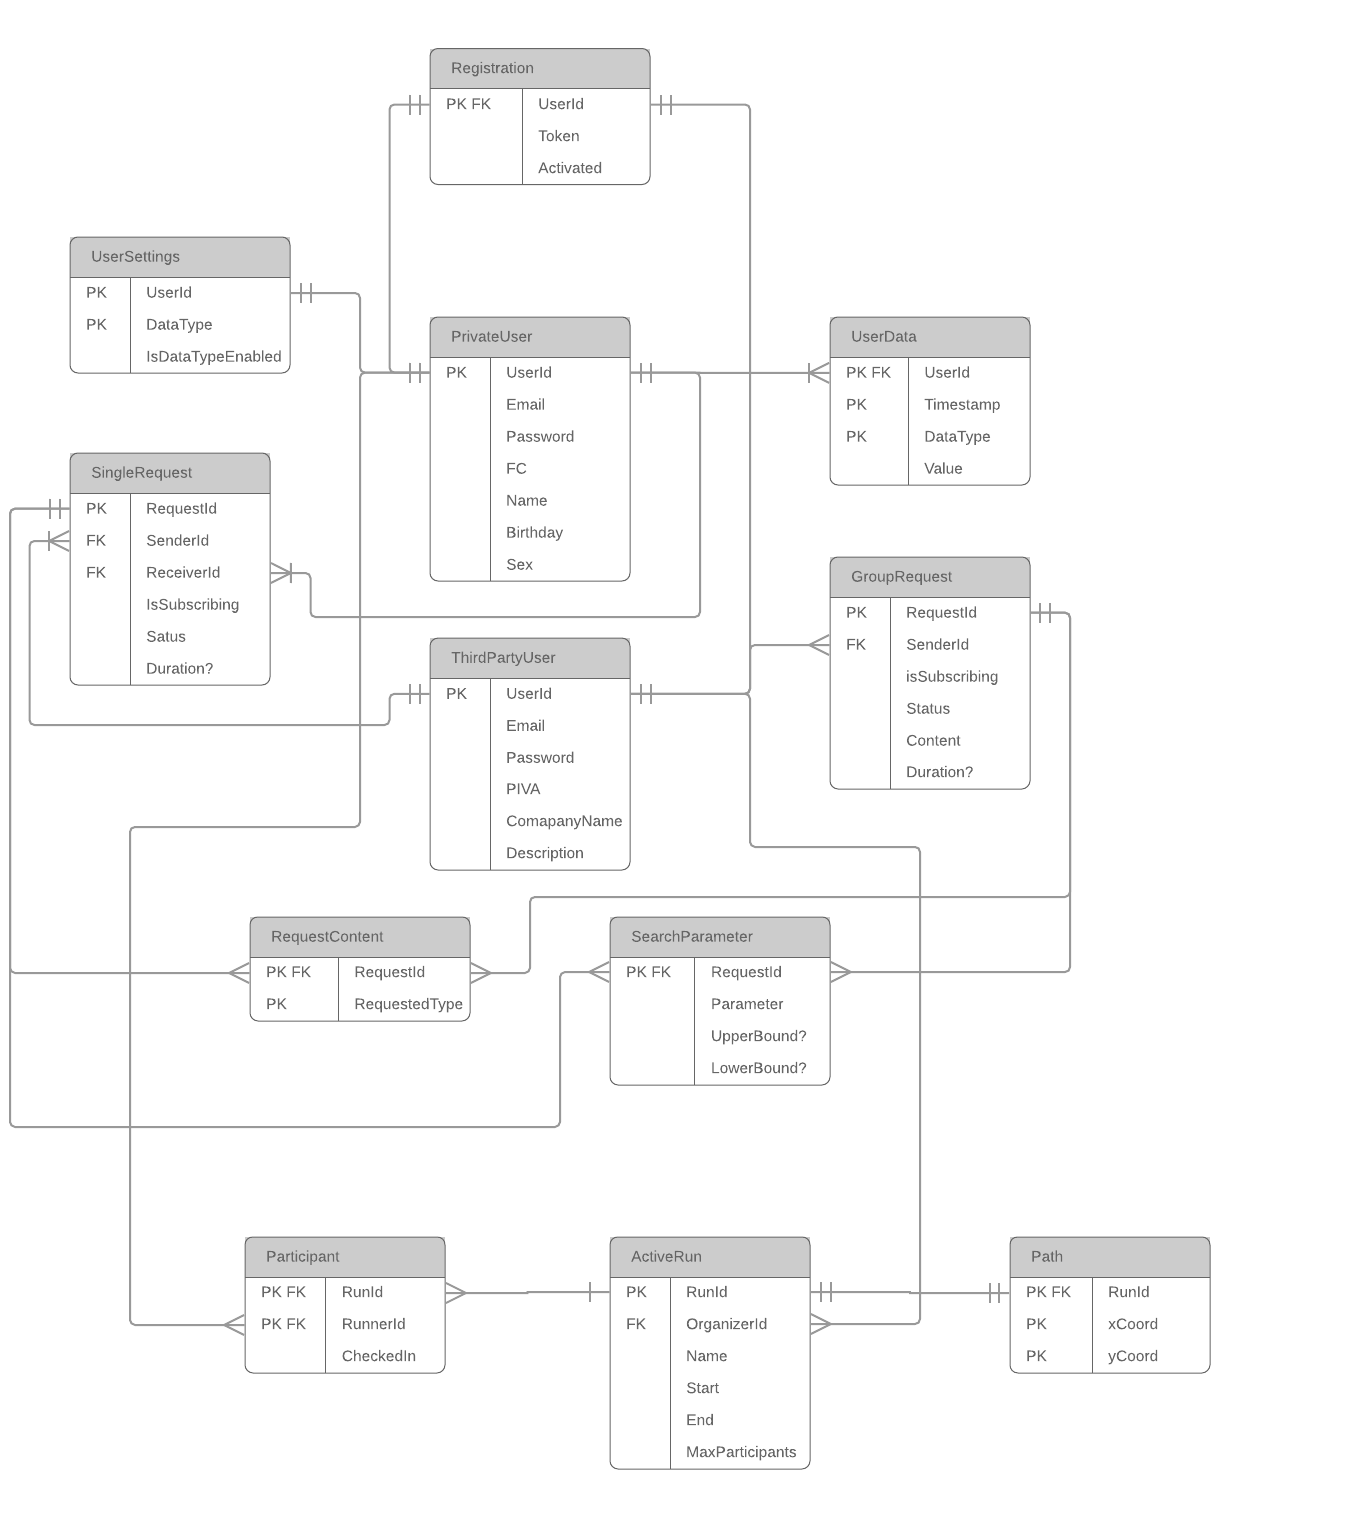
\includegraphics[width=15cm]{ER.png}
  	\caption{Entity-Relationship diagram}
 	\label{fig:ER}
\end{figure}

\pagebreak

%%%%%%%%%%%%%%%%%%%%%%%%%%%%%%%%%%%%%%%%%%%%%%%%%
%%%%%%%%%%%%%%%%%%%%SECTION 3%%%%%%%%%%%%%%%%%%%%
%%%%%%%%%%%%%%%%%%%%%%%%%%%%%%%%%%%%%%%%%%%%%%%%%

\section{User Interface Design}
We already assessed the  UI design in section 3.1.1 of the RASD document. In this section, we provide a better overview about the User Experience flow by means of a User Experience diagram. The following two diagrams show the relations between the Application’s sections.
\begin{figure}[H]
	\center
  	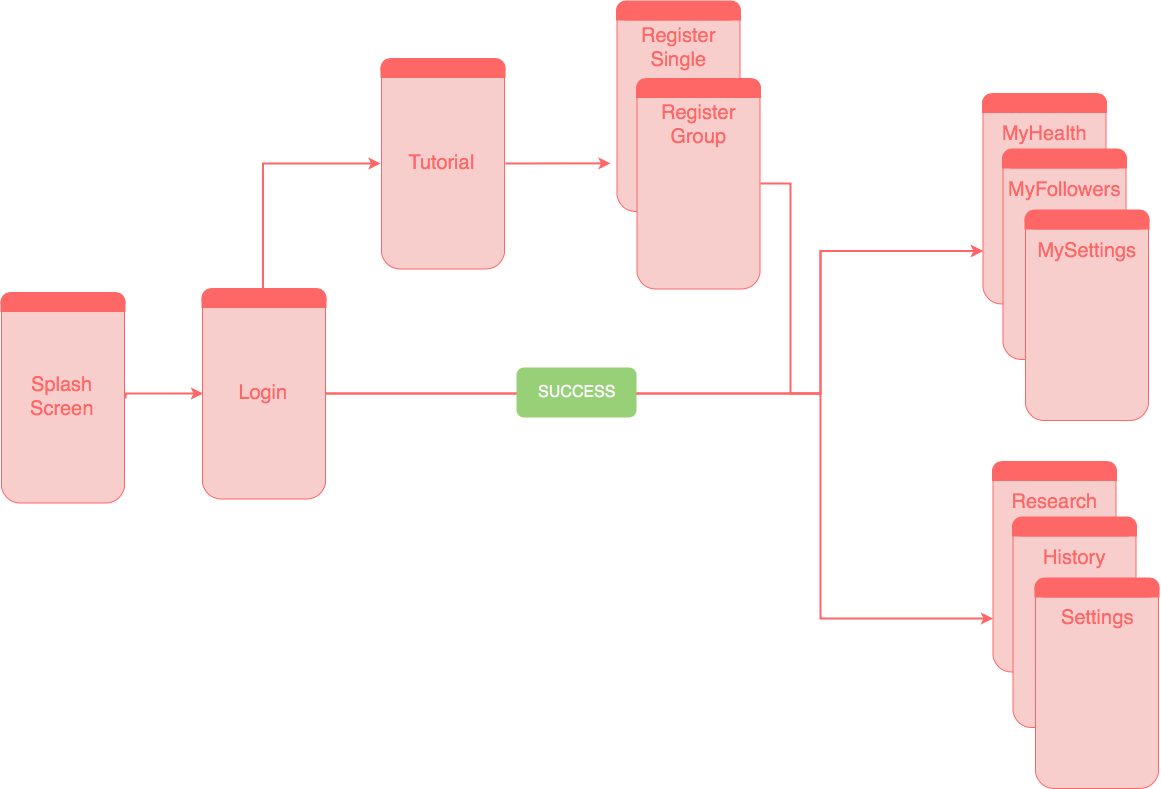
\includegraphics[width=15cm]{UXD4HDiagram.png}
  	\caption{Data4Help UX Flow}
 	\label{fig:D4HUX}
\end{figure}
\begin{figure}[H]
	\center
  	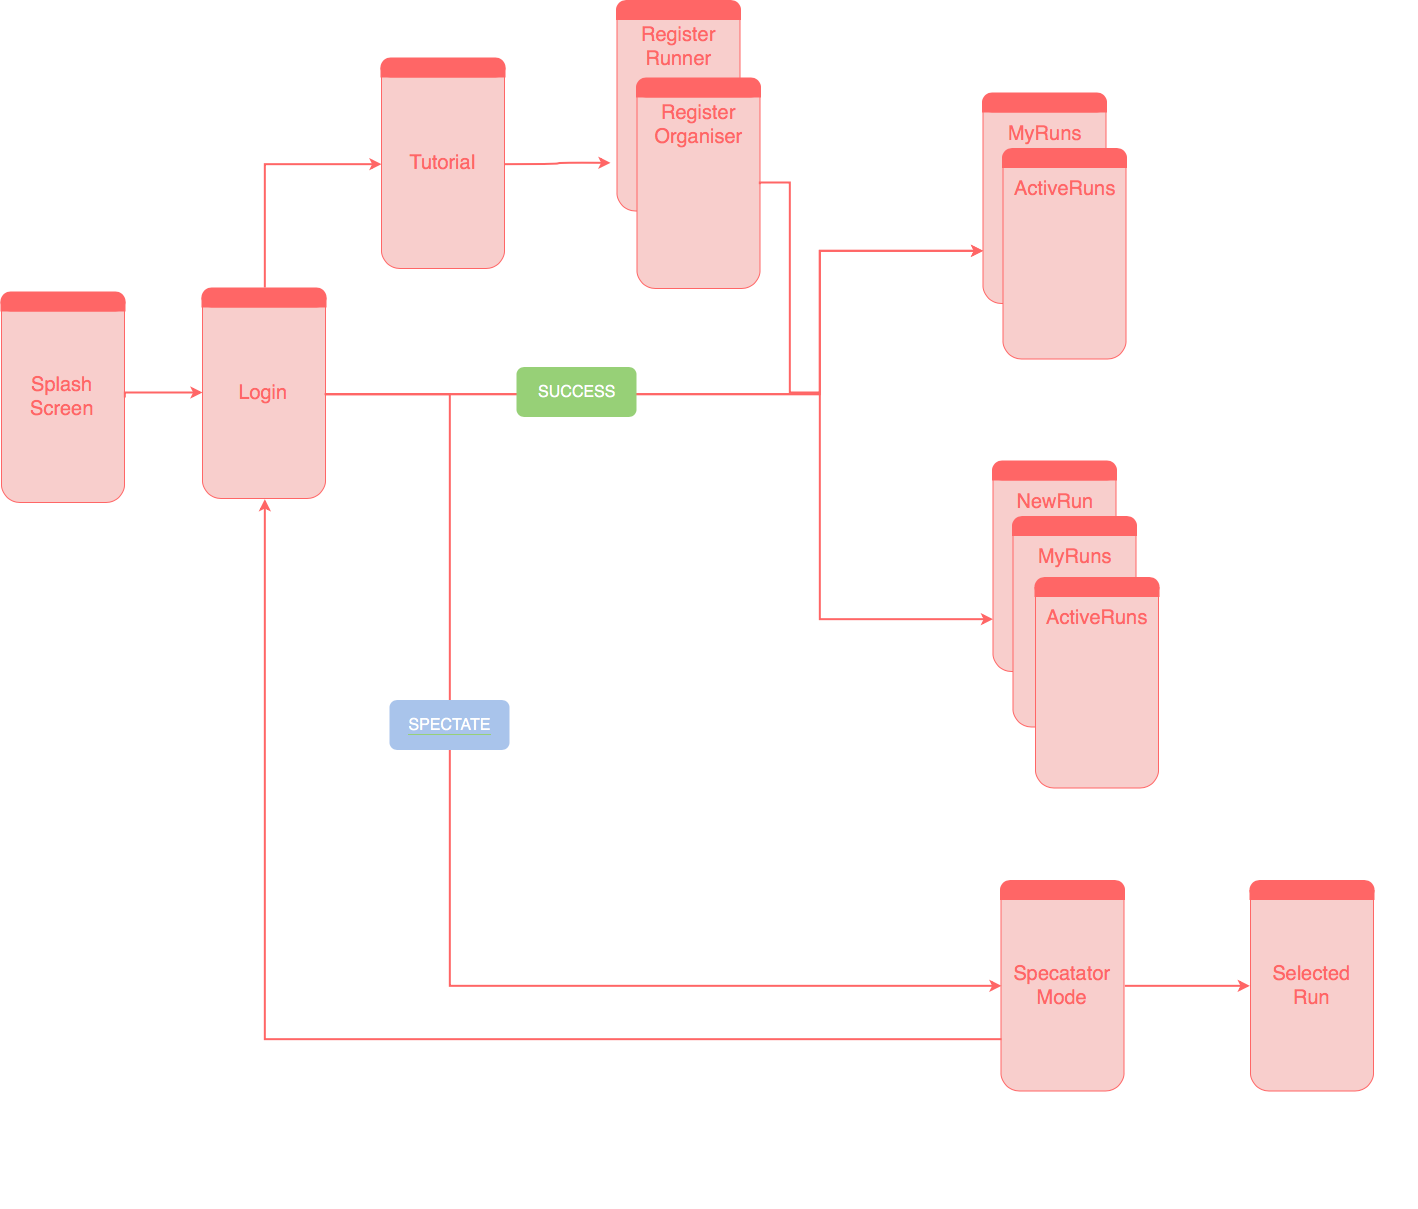
\includegraphics[width=15cm]{UXT4RDiagram.png}
  	\caption{Track4Run UX Flow}
 	\label{fig:T4RUX}
\end{figure}
\pagebreak

%%%%%%%%%%%%%%%%%%%%%%%%%%%%%%%%%%%%%%%%%%%%%%%%%
%%%%%%%%%%%%%%%%%%%%SECTION 4%%%%%%%%%%%%%%%%%%%%
%%%%%%%%%%%%%%%%%%%%%%%%%%%%%%%%%%%%%%%%%%%%%%%%%

\section{Requirements Traceability}

\begin{longtable}{| p{5 cm} | p{8 cm} |} \hline
		Component (DD) & Requirements (RASD)  \\ \hline
		\newline Authentication Manager & 
		\begin{itemize}
			\item {\bf [R1]} The S2B allows users to create either a Single User or a Third Party account. 
			\item {\bf [R2]} A Single User account can be created if and only if the user provides his Fiscal Code. 
			\item {\bf [R3]} A Third Party account can be created if and only if a valid P.IVA is provided. 
			\item {\bf [R4]} All users can create an account if and only if they provide a unique email and a password. 
			\item {\bf [R5]} To access the service users must log in with their account credentials.
			\item {\bf [R36]} The S2B allows organisers to create a Third Party account using Data4Help.
			\item {\bf [R44]} The S2B allows runners to create a Single User account using Data4Help.
		\end{itemize}	\\ \hline
		\newline Single User Manager & 
		\begin{itemize}
			\item {\bf [R33]} Only private users can choose whether or not to enable AutomatedSOS. 
		\end{itemize}		
		\\	 \hline	
		\newline Single Request Manager & 
		\begin{itemize}
			\item {\bf [R10]} Third Parties can submit a request to access data of a Single User. 
			\item {\bf [R11]} Single Requests must specify either the email or the FC of the desired user.
			\item {\bf [R12]} Single Requests are forwarded only to the specified user.
			\item {\bf [R13]} A user can accept or refuse requests forwarded to him. 
			\item {\bf [R14]} Third Parties can access user’s data if and only if their request is accepted by said user. 
			\item {\bf [R18]} Single requests must specify the requested data types. 
			\item {\bf [R19]} A request to a single user must specify whether or not the Third Party is subscribing to that request of data.
			\item {\bf [R20]} Subscriptions to requests must specify a duration.
			\item {\bf [R21]} Subscriptions to requests can be ended by both the Third Party and the single user at any time.
			\item {\bf [R22]} If none of the requested data types of the single user is available, the Third Party receives an error message.
			\item {\bf [R23]} Third Parties can access only the requested data types that are available.
			\item {\bf [R24]} Third Parties can download all data obtained through requests on their devices or have it sent by email.
			\item {\bf [R40]} The request is sent on behalf of the organiser using its email and P.IVA.
			\item {\bf [R41]} The request sent is with a subscription that lasts until the end of the run.
			\item {\bf [R42]} The request sent by the S2B has as requested data types the position and all available health parameters of the user.
			\item {\bf [R48]} A user can’t accept the request if he doesn’t have at least his position available as requestable data type.
		\end{itemize}		
		\\	 \hline	
		\newline Group Request Manager & 
		\begin{itemize}
			\item {\bf [R20]} Subscriptions to requests must specify a duration.
			\item {\bf [R24]} Third Parties can download all data obtained through requests on their devices or have it sent by email.
			\item {\bf [R25]} Third Parties can submit a group request to access data of groups of users. 
			\item {\bf [R26]} Group requests must include at least one search parameter. 
			\item {\bf [R27]} Group requests must specify the requested data types. 
			\item {\bf [R28]} Group request results are provided if and only if the number of users matching the search parameters is higher than 1000. 
			\item {\bf [R29]} Group request results include only the data retrieved by the System matching the search parameters. 
			\item {\bf [R31]} All group requests must specify whether the Third Party is subscribing to that request of data. 
			\item {\bf [R32]} Subscriptions to requests can be ended by the Third Party at any time.
		\end{itemize}		
		\\	 \hline
		\newline Data Storage Manager & 
		\begin{itemize}
			\item {\bf [R30]} Sensitive data is excluded from group request results. 
		\end{itemize}		
		\\	 \hline	
		\newline Data Manager (Client) & 
		\begin{itemize}
			\item {\bf [R7]} The S2B automatically imports new data whenever the application is opened.
			\item {\bf [R8]} When the application is open, the S2B continuously import data in background.
		\end{itemize}		
		\\	 \hline	
		\newline Data Manager (Server) & 
		\begin{itemize}
			\item {\bf [R7]} The S2B automatically imports new data whenever the application is opened.
			\item {\bf [R8]} When the application is open, the S2B continuously import data in background.
			\item {\bf [R9]} The S2B binds collected data only to the user’s account that imported it. 
		\end{itemize}		
		\\	 \hline	
		\newline Health Status Manager & 
		\begin{itemize}
			\item {\bf [R15]} The S2B allows Single Users to visualise their historical data using Time Series. 
			\item {\bf [R16]} The S2B allows Single users to visualize their historical data using aggregated statistical operators. 
			\item {\bf [R17]} The S2B allows Single users to visualize their historical data over multiple timespans.
		\end{itemize}		
		\\	 \hline
		\newline {\it AutomatedSOS} Manager & 
		\begin{itemize}
			\item {\bf [R33]} Only private users can choose whether or not to enable AutomatedSOS. 
			\item {\bf [R34]} AutomatedSOS can be enabled only if the user grants permission to make emergency phone calls. 
			\item {\bf [R35]} If AutomatedSOS is enabled and the System detects that a user’s heart rate is below or above the critical threshold for his age, an ambulance is called. 
		\end{itemize}		
		\\	 \hline
		\newline Run Manager & 
		\begin{itemize}
			\item {\bf [R37]} Only Third Parties can create a run.
			\item {\bf [R38]} When creating a run, the organiser must specify its the path, duration and maximum participants.
		\end{itemize}		
		\\	 \hline	
		\newline Active Runs Manager & 
		\begin{itemize}
			\item {\bf [R39]} On the day of a run the S2B sends a Single Request to every user who has registered to that run.
			\item {\bf [R40]} The request is sent on behalf of the organiser using its email and P.IVA.
			\item {\bf [R43]} The S2B provides a list of all existing runs visible to everyone using Track4Run.
			\item {\bf [R45]} Only users with a Single User account can join an existing run.
			\item {\bf [R46]} A user can only join a run in the list provided by the S2B.
			\item {\bf [R47]} A user can’t check-in for a run if he doesn’t accept the request received by the organiser of such run.
			\item {\bf [R48]} A user can’t accept the request if he doesn’t have at least his position available as requestable data type.
			\item {\bf [R49]} If a user fails to check-in in the run, the S2B removes him from it.
			\item {\bf [R50]} An existing run can be spectated without logging in the System.
			\item {\bf [R51]} An existing run can be spectated by selecting it in the list of existing runs.
			\item {\bf [R52]} Spectators can see the live position of all runners participating in the run they are spectating.
		\end{itemize}		
		\\	 \hline		
		\caption{Requirements Traceability}	
						
	\end{longtable}

\pagebreak

%%%%%%%%%%%%%%%%%%%%%%%%%%%%%%%%%%%%%%%%%%%%%%%%%
%%%%%%%%%%%%%%%%%%%%SECTION 5%%%%%%%%%%%%%%%%%%%%
%%%%%%%%%%%%%%%%%%%%%%%%%%%%%%%%%%%%%%%%%%%%%%%%%
\section{Implementation, Integration and Test Plan}
\subsection{Overview}
The approach followed in the design of the S2B was Top-Down, first defining the subsystems and their macro functionalities at a high abstraction level, and then refining each one up to methods and parameters needed. 
The subsystems we identified are:
\begin{itemize}
    \item The client subsystem, containing the presentation and the components related to AutomatedSOS and data retrieval
    \item The server subsystem, containing most of the components related to Business Logic and interaction with the database
    \item External services, such as the DB and the Maps service
\end{itemize}
However our implementation and testing approach will be incremental and will follow both top-down and bottom-up strategies as they are the most reasonable for relatively small components and subsystems. In the following paragraphs we will detail our strategies and discuss their advantages. 

\subsection{Implementation}
The order of implementation takes into account the necessity of parallelizing the workload between developers, and can be identified as:
\begin{enumerate}
    \item Setup of the Database and creation of the schema and its constraints
    \item Implementation of the server and client subsystems at once
    \item Integration with external services
\end{enumerate}
The setup of the database will consist in the deployment of a running instance of a new database on the selected external provider. It will then follow the creation of all the tables identified in section 2.7 and of the related constraints. \newline
\newline
The implementation of the Server and Client will proceed in parallel to optimize the efficiency between developers.
\newline
\newline
On the server side the implementation will follow this order:
\begin{itemize}
    \item Data Storage Manager, Network Manager
    \item Auth Manager, Settings Manager
    \item Single User Manager, Third Party Manager, DataManager
    \item Single Request Manager, Group Request Manager
    \item Privacy Manager
\end{itemize}
In particular Data Storage Manager and Network Manager will be implemented first because they represents the access point to the Clients and the DB and eventual changes in the structure of the interaction between the various subsystems would have repercussions on all other components.
\newline
\newline
On the client side the implementation will follow this order:
\begin{itemize}
    \item UI Components, Views
    \item NetworkManager
    \item {\it AutomatedSOS}, ViewControllers, DataManager
\end{itemize}
The DataManager component represents one of the most critical part of the Systems thus it will be immediately tested to check the interaction with the Health Monitoring Service.

\subsection{Unit testing}
During the whole duration of the implementation phase unit tests will be performed in order to spot as soon as possible bugs and flaws inside system components. Performing unit tests during the implementation of single software components is essential to be able to fix bugs with the lowest cost of repair in terms of effort and time and it also helps guiding the design of the system.
Unit tests will be added incrementally as new code is written. A support tool will be used to perform their execution automatically once a new version of the software is available. An automated test tool will be used for two reason. Firstly, it saves time for developers that do not have to manually perform all tests every time they add or change something. Secondarily, it allows to make sure that a test that was valid for a previous version of the code still holds after some changes/additions in order to preserve consistency and compatibility.
Unit tests on components will mainly focus on exercising interfaces, internal behaviour (e.g initialization) and modules’ interaction. Regarding this last aspect, the only way to make components work even in isolation is to simulate the ones that are missing. Drivers will be used to simulate calls to a certain component. Stubs will be used to simulate the calls made by a component under testing.
\begin{figure}[H]
	\center
  	\includegraphics[width=5cm]{testScaffolding.png}
  	\caption{Test scaffolding}
 	\label{fig:testScaffoling}
\end{figure}

\subsection{Integration testing}
Once we have defined how we will approach the implementation of each component of our system and how to test it independently, we shall focus on how to test their interaction and validate their joint behavior. Integration between components means testing groups of components that depend on one another in order to assess their interaction and possibly expose any defects. We will perform integration testing at two different levels: at subsystem level, meaning between components of the same macro system such as modules of the Controller or of the View, and at a system level, linking all systems together.
\newline
\newline
As previously mentioned, subsystem integration will be performed within a macro system and will follow an incremental approach as done during implementation and testing. This approach will follow a top down procedure according to the use hierarchy of modules. Previously created stubs in fact will be now substituted by real components. The only stubs and drivers we will use in this type of integration will be those of the Client (driver), the DBMS(stub). We will adopt this approach both for Data4Help and Track4Run’s architectures. In order, we will first integrate the first two levels of the use hierarchy and proceed until the very last that is composed by the Data Storage Manager, the component with functions that are called by all other components and that interacts with external services. 
\newline
\newline
The following diagram represents the use hierarchy of modules within the Data4Help’s server. As already mentioned, the order of integration we have opted for follows modules from the root to the leaves.
\begin{figure}[H]
	\center
  	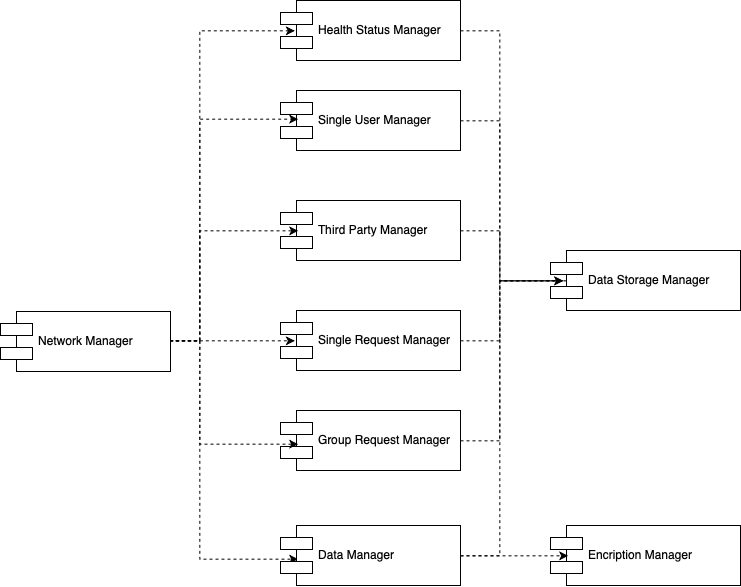
\includegraphics[width=5cm]{serverSubsystemTesting.png}
  	\caption{Server Subsystem testing}
 	\label{fig:serverSubsystemTesting}
\end{figure}
The following diagram instead contains the use hierarchy within the Data4Help client and shows our integration flow (from the root to the leaves).
\begin{figure}[H]
	\center
  	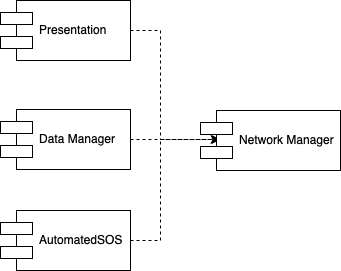
\includegraphics[width=5cm]{clientSubsystemTesting.png}
  	\caption{Client Subsystem testing}
 	\label{fig:clientSubsystemTesting}
\end{figure}
As mentioned above, the same approach will be adopted with Track4Run’s subsystems.
\newline
\newline
After having integrated each component within a system, we will focus on integrating all systems together. Our strategy in this case will be a bottom up approach based on the use hierarchy. At the very bottom level there is the Model of our system, the first element that we have created and that is interrogated by all other modules. At first we shall integrate Controller and Model in order to test calls from the former to the latter. When integrating these two components we will also use Postman to simulate client requests. This service is a simple JavaScript code that enables us to send API requests instead of having a complete Client to interact with. 
Afterwards we will add the Client to our previously integrated systems and verify the complete functioning of our system. The Client corresponds to the root of our hierarchy as it interacts only with the controller that handles its requests and communicated with the database.
Finally, when performing system integration, we will also include external service, such as Map Service, Health Monitoring Service or Push notification Service. Those used by the Server will be integrated with it after integration with the Model. Those instead used by the Client will be included at the very end.
\newline
\newline
The following diagram represents how our system test will be performed. It is true both for Data4Help and Track4Run. Arrows represent the use hierarchy, meaning that the arrows start from modules that use those corresponding to the end points. As mentioned before, our integration procedure will begin from the leaves to the root.
\begin{figure}[H]
	\center
  	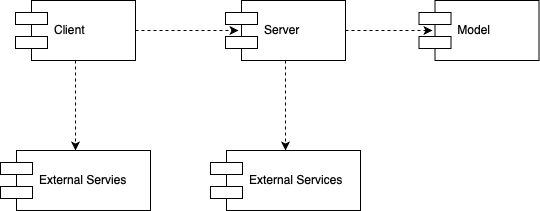
\includegraphics[width=5cm]{systemTesting.png}
  	\caption{System testing}
 	\label{fig:systemTesting}
\end{figure}
The very last step of our testing will include the integration of Data4Help and Track4Run. As previously mentioned in this document, Track4Run relies on multiple functionalities provided by Data4Help’s modules, such as those exposed by components handling requests and managing user accounts. It is then essential to test integration between the two systems in order to guarantee a seamless communication in front of the users.  
\pagebreak

%%%%%%%%%%%%%%%%%%%%%%%%%%%%%%%%%%%%%%%%%%%%%%%%%
%%%%%%%%%%%%%%%%%%%%SECTION 6%%%%%%%%%%%%%%%%%%%%
%%%%%%%%%%%%%%%%%%%%%%%%%%%%%%%%%%%%%%%%%%%%%%%%%

\section{Effort Spent}

In the following tables we will summarize the effort spent by each member of the team on the {\it DD} Document.
		
		
	\begin{longtable}{| p{2 cm} | p{5 cm} | p{2 cm} |} 
			\hline
			{\bf Date} & {\bf Task} & {\bf Hours}\\
			\hline
			19/11/18 & Pre-analysis & 2 \\
			20/11/18 & Section 1 and Latex setup & 1\\
			21/11/18 & Component View & 3 \\
			23/11/18 & Review meeting and task planning & 2 \\
			24/11/18 & RuntimeView and Overview & 4 \\
			25/11/18 & Review Component View and RuntimeView & 2 \\
			26/11/18 & Review & 1 \\
			27/11/18 & Requirements Traceability & 2 \\
			28/11/18 & Architectural Patterns & 1 \\
			04/12/18 & Group Revision & 2\\
			05/12/18 & Integration testing & 3 \\
			07/12/18 & Group revision & 2 \\
			08/12/18 & Track4Run testing & 2 \\
			08/12/18 & Final Revision & 2 \\
			08/12/18 & Copy on Latex & 2 \\
			\hline
			& & {\bf Total} \\
			\hline
			& & 31 \\
			\hline
			\caption{Virginia Negri's effort}
		\end{longtable}
	
		\begin{longtable}{| p{2 cm} | p{5 cm} | p{2 cm} |} 
		\hline
		{\bf Date} & {\bf Task} & {\bf Hours}\\
		\hline
		19/11/18 & Pre-analysis & 2 \\
		23/11/18 & Review meeting and task planning & 2 \\
		04/12/18 & Group Revision & 2\\
		07/12/18 & Group revision & 2 \\
		\hline
		& & {\bf Total} \\
		\hline
		& & 26 \\
		\hline
		\caption{Luca Molteni's effort}
	\end{longtable}
	
	\begin{longtable}{| p{2 cm} | p{5 cm} | p{2 cm} |} 
		\hline
		{\bf Date} & {\bf Task} & {\bf Hours}\\
		\hline
		17/11/18 & Purpose and Scope & 1 \\
		19/11/18 & Pre-analysis & 2 \\
		20/11/18 & DB design & 2 \\
		21/11/18 & APIs & 2 \\
		23/11/18 & Review meeting and task planning & 2 \\
		23/11/18 & APIs & 1 \\
		24/11/18 & Architectural Styles & 2 \\
		25/11/18 & RuntimeView & 3 \\
		29/11/18 & APIs review & 2 \\
		04/12/18 & Group Revision & 2 \\
		05/12/18 & Implementation & 2 \\
		07/12/18 & Group revision & 2 \\
		07/12/18 & Revision & 2 \\
		08/12/18 & Final Revision & 2 \\
		08/12/18 & Copy on Latex & 3 \\
		\hline
		& & {\bf Total} \\
		\hline
		& & 30 \\
		\hline
		\caption{Francesco Lorenzo's effort}
	\end{longtable}


\pagebreak

%%%%%%%%%%%%%%%%%%%%%%%%%%%%%%%%%%%%%%%%%%%%%%%%%

\section{References}

\end{document}